\pdfoutput=1
\documentclass[iop, apjl, twocolappendix, numberedappendix]{emulateapj}
%\usepackage{newtxtext,newtxmath}
\usepackage[T1]{fontenc}
%\usepackage{ae,aecompl}
\usepackage{float}
\usepackage{graphicx}
\usepackage{amsmath}
\usepackage{amssymb}
\usepackage{txfonts}
\usepackage{ulem}
\usepackage{xspace}
\usepackage[colorlinks=true,urlcolor=blue,linkcolor=blue,citecolor=blue]{hyperref}
%\usepackage{nccmath}
\usepackage[utf8]{inputenc}
\newcommand{\fhat}[1]{\expandafter\hat#1}
\newcommand{\fbar}[1]{\expandafter\bar#1}
\newcommand\fnurl[2]{%
  \href{#2}{#1}\footnote{\url{#2}}%
}
\def\rs{r_{\rm s}}
\def\rhos{\rho_{\rm s}}
\def\se{s_{\rm e}}
\def\ftrans{f_{\rm trans}}
\def\rhog{\rho_{\rm g}}
\def\rhoginner{\rho_{\rm g}^{\rm inner}}
\def\rhogouter{\rho_{\rm g}^{\rm outer}}
\def\rt{r_{\rm t}}
\def\rout{r_{\rm out}}
\def\mpch{h^{-1}{\rm Mpc}}
\def\msunh{h^{-1}{\rm M_{\odot}}}
\shorttitle{Splashback radius of Planck-SZ clusters}
\shortauthors{Zürcher, More \& Refregier}
\slugcomment{Master's Thesis:
In partial fulfillment of the requirements for the Master of Science ETH in Interdisciplinary Sciences}

\begin{document}

\title{The Splashback Radius of Planck-SZ clusters}

\author{
D. Zürcher \altaffilmark{1, 2}
Surhud More \altaffilmark{2, 3, 5}, 
A. Refregier \altaffilmark{4, 6}
}
\affil{
$^{1}$Department of Chemistry and Applied Biosciences, ETH Zurich, Vladimir-Prelog-Weg 1, 8093 Zurich, Switzerland;{\tt dominikz@student.ethz.ch}\\
$^{2}$Kavli Institute for the Physics and Mathematics of the Universe (Kavli IPMU, WPI), \\ 
${^3}$The University of Tokyo, 5-1-5 Kashiwanoha, Kashiwa, Chiba 277-8583\\
$^{4}$Department of Physics, ETH Zurich, Wolfgang Pauli Strasse 27, 8093 Zurich, Switzerland\\
${^5}$Supervisor\\
${^6}$Co-supervisor\\
}

%\pubyear{2018}

%\begin{document}
%\label{firstpage}
%\pagerange{\pageref{firstpage}--\pageref{lastpage}}
%\maketitle

\begin{abstract}
%Being a unique observational probe for the mass accretion rate of
%dark matter halos the splashback radius has been well-modeled by the
%use of numerical simulations. However, although its signature has
%been found using optical cluster catalogs, discrepancies from the
%simulations were noted and the plausibility of the detections were
%questioned. We overcome those caveats by using SZ selected clusters
%from the Planck survey. By cross-correlation with galaxies from the
%Pan-STARRS survey we construct the two-dimensional galaxy cluster -
%galaxy cross-correlation signal. We detect a clear steepening in the
%signal, which is steeper than $-3$ and poorly modeled by the NFW
%profile. The feature is found at a location consistent with the
%expectations. The uncertainty on the location of the splashback
%radius is recorded as $\sim 15$\%. We also study the
%cross-correlation of red and blue galaxies, separately and find
%evidence for the existence of the splashback feature in both
%populations. Further, we record a strong increase in the fraction of
%red galaxies that is associated with the splashback radius. 

We present evidence for the existence of the splashback radius
in galaxy clusters selected using the Sunyaev-Zeldovich effect.
We show that the deprojected cross-correlation of galaxy clusters
found in the Planck survey with galaxies detected photometrically in
the Pan-STARRS survey, shows a sharp steepening feature (a
logarithmic slope steeper than $-3$), which we associate with the
splashback radius.  We infer the three-dimensional splashback radius
for the SZ cluster sample to be $r_{\rm sp}=1.85_{-0.30}^{+0.26}$ $\mpch$,
where the cluster sample has an average halo mass $M_{\rm
500c}=3.0\times10^{14}\msunh$ at an average redshift of $z=0.18$.
The inferred value of the splashback radius is consistent with the
expected location for dark matter halos in the standard cold dark
matter paradigm. However, given the limited precision of our
measurements, we cannot conclusively rule out the smaller splashback
radius measured so far in the literature for photometrically
selected galaxy clusters. We show that the splashback radius does
not depend upon the galaxy magnitude for galaxies fainter than
$M_i-5\log h=-19.44$, and is present at a consistent location in
both red and blue galaxy populations. The presence of the splashback radius in
color-separated galaxy distributions could potentially be used to put lower limits on the
quenching timescales for galaxies. Further, we record a strong increase 
in the fraction of red galaxies that is associated with the splashback radius.

\end{abstract}

%\begin{keywords}
%galaxies:clusters:general -- galaxies:halos -- methods:observational -- cosmology:dark matter -- cosmology:large-scale structure of Universe -- cosmology:observations
%\end{keywords}

\section{Introduction}
\label{sec:Introduction}

The density distribution of matter within dark matter halos shapes
the potential well in which galaxies form and grow. Therefore, the
structure of these dark matter halos has been extensively studied
both theoretically as well as in numerical simulations \citep[see
e.g.,][]{gunn1972infall, fillmore1984self, bertschinger1985self,
navarro1997universal, moore1999dark}. Studies with numerical
simulations show that the density profiles of dark matter halos
within their virial radii are roughly self-similar and follow the
Navarro-Frenk-White (NFW) profile \citep{navarro1997universal},
which asymptotes to a slope of $-1$ in the inner regions and $-3$ at
large radii. There has been intense debate in the literature about
the exact form of the density profile 
\citep[e.g.,][]{navarro2004inner}, the value of the asymptotic inner slope,
as well as the outskirts and boundaries of dark matter halos
\citep{cuesta2008virialized, more2011overdensity, diemer2013pseudo}. 

The recent study of \citet{diemer2014dependence} has sparked a
renewed interest in understanding the structure of dark matter halos
on scales beyond the typical virial radii.
\citet{diemer2014dependence} investigated the outskirts of dark
matter halos in numerical simulations and found the existence of a
physical feature, namely a sharp steepening in the density
distributions of dark matter halos, which is not captured by
commonly used functional forms such as the NFW profile. They showed
that even for halos of the same mass, the position of the feature
changes depending upon the mass accretion rate of the halos. A simple
theoretical toy model to explain this feature was presented by
\citet{adhikari2014splashback}. They showed that the feature
observed by \citet{diemer2014dependence} results from the  piling up
of recently accreted dark matter particles at the apocenters of
their orbits, and its location corresponds to the last density
caustic in the self-similar models of secondary infall
\citep{fillmore1984self, bertschinger1985self, lithwick2011self}.
They coined the term ``splashback radius`` for this feature. Their
toy model also naturally explains the accretion rate dependence --
faster accreting halos have smaller splashback radii. 

%The interpretation of the dependence on accretion rate is straightforward and can be explained by the dynamics of a dark matter particle falling down and subsequently climbing out of a changing potential well of the dark matter halo. The dark matter particle will gain kinetic energy as it falls down the potential well. However if the potential well grows during this time, then the particle does not have enough energy to climb out of it. This results in the reduction of the apocenter of its orbit, and hence the splashback radius. The faster the accretion rate, the deeper the potential well gets, the smaller the splashback radius.

The interpretation of the accretion rate dependence is
straightforward. Due to the continuous change of the gravitational
potential of the halo, depending on its accretion rate, the kinetic
energy of a recently accreted dark matter particle, gained during
its infall onto the cluster, does not suffice to climb the deepened
potential well completely again, but instead it ``splashes back`` at
a distance that depends on the recent deepening of the potential
well.

Subsequently, \citet{more2015splashback} studied the
growth rate of dark matter halos at low redshift and showed that
pseudo-evolution, caused by the ill-definition of the halo boundary
through the virial radius, accounts for nearly all of the apparent
growth of galaxy-sized halos and can also account for a substantial
fraction of the growth of cluster-sized halos
\citep{diemer2013pseudo}. They suggested the use of the splashback
radius as a natural boundary for dark matter halos and explored its
consequences for the inferred boundaries and growth rates of the
halos.  It was found that depending on the accretion rate of the
halo, the splashback radius may lie well beyond the commonly used
virial radius. For quickly accreting halos the splashback radius is
expected to occur at $\approx 0.8-1$ $r_{\mathrm{200m}}$ and at
$\approx 1.5$ $r_{\mathrm{200m}}$ for slowly accreting halos
\citep{more2015splashback}.

Given the mass of the halo, the location of the splashback radius
constitutes a direct probe of the halo accretion rate. Motivated by
these studies, \citet{more2016detection} tried to detect this
feature in observations. Using the optically selected Sloan Digital
Sky Survey RedMaPPer galaxy cluster catalog
\citep{rykoff2014redmapper}, and by cross-correlating it with the
SDSS photometric galaxy sample, \citet{more2016detection} found evidence
for the steepening of the dark matter density profile, and therefore
the splashback radius of this sample of galaxy clusters (later
corroborated by including further models for mis-centering by
\citet{baxter2017halo}). Somewhat surprisingly,
\citet{more2016detection} found that the location of the splashback
radius was inconsistent with that expected from numerical
simulations of dark matter by about $20\pm5$\%. Although they
investigated potential systematic issues, they did not have access
to mock cluster catalogs which could mimic the selection effects of
optically-identified clusters. \citet{busch2017assembly} used a
simplified optical cluster selection algorithm on the Millennium
simulation, and pointed out that optical clusters can be heavily
affected by projection issues, and could potentially introduce
systematics in the inference of the splashback radius, as well as
halo assembly bias. The existence of projection effects in the
optical cluster catalog in the context of halo assembly bias was 
also demonstrated by \citet{zu2016level}.

\citet{umetsu2017lensing} used Xray selected clusters to look for
the splashback radius using the weak lensing signal, however
stacking issues and the low signal-to-noise ratio remains a significant
hurdle. \citet{chang2017splashback} find evidence for the splashback
radius in the weak lensing signal, but their analysis was again done
using optically selected clusters in the Dark energy survey
\citep{dark2005dark}. Regardless of the projection issues present in
the optical cluster catalog, there is some inherent circularity
present in the logic of using photometric galaxies to select
clusters as over-densities in a given aperture, and then using the
same photometric sample of galaxies to look for the splashback
radius. There is a possibility that the aperture used to select the
cluster catalogs could be imprinted in a non-trivial way on the
measured number density profiles of clusters. 

In this work, we move away from the optical cluster selection and
explore the use of SZ selected cluster catalogs. While the SZ
selected clusters can also be susceptible to systematic selection
effects, the scales on which the SZ signal is measured and the
cluster selection is performed is much smaller than the expected
location of the splashback radius. Therefore, we do not expect major
systematic biases due to the selection process. We use this sample
to explore the evidence for the splashback radius in observations.
Due to the low signal-to-noise ratio of the weak lensing signal, we
perform our analysis using cross-correlation of galaxies with
clusters instead. The SDSS sample used by \citet{more2016detection}
was deep enough such that biases in the location of the splashback
radius due to dynamical friction effects were expected to be small.
Nevertheless, we use galaxy samples, which are even fainter by
$0.5-1$ magnitudes compared to those used by
\citet{more2016detection}.

%The correct interpretation of observations of large scale structures in the universe requires accurate, theoretical predictions for the structure of dark matter halos as they form in a cold dark matter scenario. Therefore, a large efford has been made in the past decades to predict the density profiles of dark matter halos starting with \citet{gunn1972infall} who used a simple top hat model to describe the collapse of the halos. However, cosmolgical simulations revealed that the collapse of the halos are rather triaxial than spherically symmetric and therefore more complicated than expected \citep{klypin1983three}. The NFW profile named after its inventors \citet{navarro1997universal} became one of the most popular models taking into account the triaxial nature of the collapse. It was found that the profiles of dark matter halos exhibit a monotonical steepening at larger radii \citep{huss1999universal}. This behaviour is badly described by the NFW profile which inherits an asymptotic slope of -3 at large radii, since \citet{navarro1997universal} focused on the description of the inner part of the dark matter halos. Instead, a more accurate desription has been found through the Einasto profile (e.g., \citep{navarro2004inner}).
%Most of the studies on dark matter halo profiles focused on the inner regions of halos since these are more easily probed by the observable galaxy distributions (e.g., \citep{moore1999dark}). However, through X-Ray and Sunyeaev-Zeldovich surveys as well as weak gravitational lensing studies the mass distribution of the outskirts of the halos become more and more accesible \citep{diemer2014dependence}. Therefore, \citet{diemer2014dependence} investigated the outer regions of the dark matter halos in order to provide more accurate models for the description of the outskirts of the halos which are necessary for the correct interpretation of such observations. They showed, that the classical fitting functions such as the NFW or the Einasto profile fail to describe the outer parts of the mass profiles as inferred from N-body simulations. Particularly they found a sharp steepening of the profile around the virial radius $r \approx r_{\mathrm{200m}}$, which is not modeled correctly by those fitting functions and they argue that the local steepening is caused by a caustic formed by recently accreated particles which passed through the pericenter of their orbit just once since their infall onto the cluster. They proposed a new fitting function consisting of an inner Einasto profile and an outer power law profile connected by a smooth transition
%\begin{align}
%\rho(r) &= \rho_{\mathrm{in}}(r)f_{\mathrm{trans}}(r) + \rho_{\mathrm{out}}(r)\,, \\
%\rho_{\mathrm{in}}(r)&=\rho_{\mathrm{s}}\exp\left( -\frac{2}{\alpha}\left[ \left( \frac{r}{r_{\mathrm{s}}}\right)^{\alpha}-1 \right] \right)\,,\\
%\rho_{\mathrm{out}}(r)&=\rho_{\mathrm{0}}\left( \frac{r}{r_{\mathrm{out}}}\right)^{-s_{\mathrm{e}}} \,,\label{eq:model} \\
%f_{\mathrm{trans}}(r)&=\left( 1+\left( \frac{r}{r_{\mathrm{t}}} \right)^{\beta} \right)^{-\gamma/ \beta}\,,
%\label{eq:dk14}
%\end{align}
%where $r$ indicates the three dimensional radial distance from the halo center \citep{diemer2014dependence}.

%In a follow up study \citet{adhikari2014splashback} derived a simple theoretical model from first principles explaining the presence of the local steepening found by \citet{diemer2014dependence}. They base their work on the ideas developed by \citet{diemer2014dependence} and \citet{fillmore1984self}. They argue that caustics arise in triaxial collapses of dark matter due to a pile up of the orbits of multiple particles at a similar radius. Such caustics most frequently appear close to the apocenters of the orbits due to the radial velocity being very small at that point, which causes the particles to spend a longer time there \citep{lithwick2011self}. The outermost caustic of a halo is associated with the first apoapsis of the most recently accreted particles. Those particles underwent a first collapse meaning that they passed through the center of the halo just once. This phenomenon is termed splashback effect and the radius corresponding to the density drop after the outermost caustic has been named splashback radius correspondingly. 

%The location of the splashback radius strongly depends on the accretion rate $\Gamma$ of the halo. The interpretation of the dependence on $\Gamma$ is straightforward: Imagine a dark matter particle which passed through the center of the halo just once and is on its way back towards larger radii. If the gravitaional potential of the halo would be static the particle would inherit enough kinetic energy to climb the potential and leave the halo again. However, since the halo keeps on accreating matter while the particle moves away from the center, its gravitational potential well deepens and the dark matter particle will not be able to climb the potential completely but instead "splashes back" towards the center of the halo. The deepening of the potential during the particle's journey depends on the amount of the accreated material and therefore on the value of $\Gamma$. Hence, a larger $\Gamma$ leads to a smaller splashback radius. This means that the location of the splashback radius can be used to infer the accretion rate of a halo \citep{adhikari2014splashback}

%Similarly, the redshift dependence arises through the influence of the values of the cosmological paramerters $\Omega_m$ and $\Omega_{\Lambda}$ on the amount of material that can be accreated onto the halo during the time that the particle requires to travels outwards from the center again. At lower redshifts $\Omega_m$ decreases quickly as $\Omega_{\Lambda}$ becomes more dominant. Therefore, the mean background density $\bar{\rho}_m$ of the universe decreases quickly as well and the halo can only accreate less and less material which slows down the deepening of the potential well and increases the splashback radius \citep{adhikari2014splashback}.

%Motivated by the collapse model of a spherical top-hat over-density the outer boundary of a halo is usually defined as a radius $R_\Delta$ enclosing a region with an over-density of $\Delta$ or more with respect to a certain reference density $\rho_{\mathrm{ref}}$, where the lower bound of the required over-density is given from the virialization criterion at the time of the virialization of the halo \citep{gunn1972infall}. However, \citet{diemer2013pseudo} found that such a boundary definition can lead to pseudo-evolution of the halo mass, meaning an apparent growth of the halo mass that is caused only by the evolution of the reference density with redshift and not by a physical accretion of mass onto the halo. Using simulations they showed that pseudo evolution accounts for nearly all of the apparent growth between $z=1$ and $0$ of galaxy-sized halos and can also account for a substantial fraction of the growth of cluster-sized halos \citep{diemer2013pseudo}. Further, \citet{diemer2013pseudo} realized that a new definition for the boundary of halos is required which must not suffer from pseudo-evolution. \citet{more2015splashback} proposed to use the newly discovered splashback radius as such an alternative definition. They found that depending on the accretion rate of the halo, the splashback radius may be well beyond the commonly used virial radius. For quickly accreting halos the splashback radius is expected to occur at $\approx 0.8-1$ $r_{\mathrm{200m}}$ and at $\approx 1.5$ $r_{\mathrm{200m}}$ for slowly accreting halos \citep{more2015splashback}.

%Cross-correlating the Sloan Digital Sky Survey (SDSS) Data Release 8 (DR8) photometric galaxy catalog with clusters identified from the SDSS DR8 catalog by the redMaPPer algorithm \citep{rykoff2014redmapper,rozo2015redmapper} \citet{more2016detection} presented evidence for the existence of the splashback radius in observations. By studying the stacked surface density profiles of the galaxy clusters they detected a sharp steepening providing strong evidence for the existence of the splashback effect. 

%\citet{more2016detection} compared their findings with simulations by utilizing the MultiDark-Planck II N-body simulation \citep{klypin2016multidark}. The comparison showed that the splashback radii detected are smaller than expected from the simulation. They explored several systematic effects which could lead to such deviations. However, none of the investigated, systematic effects can account for the discrepancies found in the data. 

Given that the splashback radius represents a true halo boundary,
the observations of the splashback radius can be used to study a
variety of galaxy formation questions. Such as questions 
regarding the timescales and the spatial scales within
which star forming galaxies quench after they fall into the cluster
potential. Answers to those questions are important to understand 
the evolution of satellite galaxies in massive galaxy clusters. 
If blue galaxies quench before
they complete a single orbit, then they are not expected to show a
splashback feature in their density distribution. In pursuit of this
question, we also explore the dependence of the cluster-galaxy
cross-correlations separately for the red and blue galaxies and
explore their relative contributions to the overall density profile.

This paper is organized as follows: Section~\ref{sec:Methods} starts
by introducing the data, namely the cluster and the galaxy catalogs
as well as the methods that are used to derive the results which are
presented in visual and tabular form and  discussed in
Section~\ref{sec:Results}. We outline the steps that will be taken
in future works in Section~\ref{sec:Future} and finally we summarize
our findings in Section~\ref{sec:Conclusions} and provide a short
outlook on what needs yet to be done. Throughout the paper, we use a
flat $\Lambda$CDM cosmology with $\Omega_{\rm m}=0.27$ to convert
redshifts and angles into cosmological distances. Also, we denote 
three-dimensional distances by $r$ and projected distances by $R$.


\section{Data and Methods}
\label{sec:Methods}
The methodology we adopt for locating the splashback radius closely
follows \citet{more2016detection}. We perform a cross-correlation
between SZ selected galaxy clusters with photometric galaxies in
order to assess the existence and location of the splashback radius.
We describe the data sets we use and our methodology in this
section.


\subsection{Cluster catalog}
\label{sec:clusters}
The baryonic component of a galaxy cluster is dominated by the hot,
ionized  intra-cluster medium (ICM), which is gravitationally bound
within the cluster. The cosmic microwave background (CMB) photons
that pass through the cluster inverse Compton scatter off the hot
electrons and gain energy. This effect is known as the thermal
Sunyaev-Zeldovich (SZ) effect
\citep{sunyaev1970small,sunyaev1980velocity}. The effect has a
characteristic frequency dependence and results in an intensity
decrease below 220 GHz and an associated increase at higher
frequencies. The multiple frequency channels on the Planck satellite
allow a detection of galaxy clusters using the SZ effect
\citep{collaboration2016planck}. As part of the 2015 Data Release of
the Planck mission, the second Planck Catalogue of Sunyaev-Zeldovich
Sources (PSZ2) was made available to the community. The PSZ2 catalog
contains detections based on  three different techniques
\citep{ade2016planck}, and the union of these catalogs has in total
1653 galaxy clusters, of which 1203 clusters have been confirmed by
cross-matching to other galaxy clusters from external data sets. 
%what 3 techniques???
\begin{table}
    \centering
    \caption{Comparison of the PSZ2 cluster catalog
    against the RedMaPPer cluster catalog used by
\citet{more2016detection}. The values of the mass estimates
$M_{\mathrm{500c}}$, $M_{\mathrm{200m}}$, redshifts $z$ and expected
splashback radii $r^{\mathrm{3D,theo}}_{\mathrm{sp}}$ represent the
catalog averages. The redshifts for both catalogs are given from the
survey. For the RedMaPPer catalog the $M_{\mathrm{200m}}$ mass
estimates were obtained from gravitational lensing and for the PSZ2
catalog the $M_{\mathrm{500c}}$ estimates were calculated from the
survey parameters using the scaling relation between the integrated
Compton Y-parameter $Y_{500c}$ and $M_{500c}$ as found by
\citet{ade2014planck}. The missing mass estimates as well as the
expected values of the splashback radii were calculated using the
Python package COLOSSUS \citep{diemer2017colossus}. The predictions
for the splashback radii $r^{\mathrm{3D,theo}}_{\mathrm{sp}}$ is
given in comoving units.}
    \label{tab:cluster_catalogs} 
    \begin{tabular}{ccc}
    \hline 
    & RedMaPPer & PSZ2 \\
    \hline 
    $z$ & 0.24 & 0.177 \\
    \hline 
    \# objects & 8643 & 596\\
    \hline
    $M_{\mathrm{500c}}$ [$h^{-1}10^{14} $M$_{\sun}$] & 0.9 & 3.0 \\
    \hline
    $M_{\mathrm{200m}}$ [$h^{-1}10^{14} $M$_{\sun}$] & 1.8 & 6.2\\ 
    \hline
    $r^{\mathrm{3D,theo}}_{\mathrm{sp}}$ [$h^{-1}$ Mpc] & 1.37 & 1.89 \\
    \hline
    \end{tabular} 
\end{table}
\begin{table*}
    \centering
    \caption{Summary and comparison of the properties of the galaxy catalogs used in this work as well as the SDSS catalog used in \citet{more2016detection}.}
    \label{tab:galaxy_catalogs}
    \begin{tabular}{ccccc}
    \hline 
    & SDSS & PS 21 & PS 21.5 & PS 22 \\ 
    \hline 
    depth [mag] & 21.00 & 21.00 & 21.50 & 22.00\\ 
    \hline 
    eff. area [deg$^2$] & $\approx$ 10'000 & 21'148 & 20'586 & 15'689\\ 
    \hline 
    \# objects & 57'181'113 & 93'772'329 & 123'188'529 & 105'809'113 \\
    \hline
    objects/deg$^2$ & 5718 & 4434 & 5984 & 6744\\ 
    \hline
    \end{tabular} 
\end{table*}
\begin{table*}
    \centering
    \caption{Summary of the priors used in the MCMC sampling
procedure. The MCMC chains are constrained using flat priors or
normal priors on some of the fitting parameters. This table lists
the ranges of the flat priors and the central positions as well as
the scales of the normal priors ( format: center | scale ),
respectively.}
    \label{tab:priors}
    \begin{tabular}{ccccccccc}
    \hline 
    & $\log_{10}(\rho_{\mathrm{s}})$ & $\log_{10}(\alpha)$ & $\log_{10}(r_{\mathrm{s}})$ & $\rho_0$ & $s_{\mathrm{e}}$ & $\log_{10}(r_{\mathrm{t}})$ & $\log_{10}(\beta)$ & $\log_{10}(\gamma)$ \\ 
    \hline 
    %$\mathrm{Var}_{\mathrm{init}}$ & 0.8 & 0.030 & 0.058 & $4.7\cdot10^{-6}$ & $3.8\cdot10{-7}$ & 0.0088 & 0.25 & 0.0078\\ 
    %\hline 
    Prior Type & None & Normal & Flat & None & None & Flat & Normal & Normal\\ 
    \hline 
    Prior Range & - & $\log_{10}(0.2)| 1.2$ & [0.1,5.0] & - & - & [0.1,5.0] & $\log_{10}(6.0) | 0.4$ & $\log_{10}(4.0) | 0.4$\\
    \hline
    \end{tabular} 
\end{table*}

The 1-$\sigma$ errors on the cluster positions are $\sim1.6\arcmin$
and the estimated purity of the catalog has a lower limit of 83\%
(probability that a detection corresponds to a real object). The
integrated Compton Y-parameter $Y_{500c}$ of each of the clusters
are also provided. Based on the scaling relation between $Y_{500c}$
and $M_{500c}$ \citep{ade2014planck} the mass estimates $M_{500c}$
of the clusters are calculated
\citep{adam2016planck,collaboration2016planck}. The PSZ2 union
cluster catalog is publicly available from the \fnurl{\textit{Planck
Legacy Archive}}{https://pla.esac.esa.int/pla/\# home}.

We restrict ourselves to the redshift range $0.03 \leq z \leq 0.33$
in order to mimic the redshift range used by
\citet{more2016detection}. Due to the large beam size of the Planck
satellite, the cluster positions as reported in the catalog may be
mis-centered from the true center of the galaxy clusters. We perform
a visual inspection of Pan-STARRS images taken around the detected
galaxy clusters in order to locate the nearest, brightest cluster
galaxy (BCG). We regard the position of the BCG as the true cluster
location, under the assumption that the BCG is located at the true,
gravitational center. The final sample that we use consists of 596
galaxy clusters and is about an order of magnitude smaller compared
to the sample used in \citet{more2016detection}. The sample we use
in this paper has an average redshift of 0.177, and an average
cluster mass $M_{500c}$ of about $3.0 \cdot 10^{14}
h^{-1}$M$_{\sun}$. In Table~\ref{tab:cluster_catalogs} we compare
the main properties of the cluster catalog used in this work to that
used by \citet{more2016detection}. The sky positions of the clusters
can be found in Figure~\ref{fig:planck_fig} in
Appendix~\ref{sec:figures}. 

\citet{kosyra2015environment} found no evidence for a significant
correlation between the density of Planck detections and the
weighted average noise of all Planck channels at $z<0.5$. Since we
restrict ourselves to $z<0.33$, we utilize the selection mask of the
PSZ2 union catalog in order to construct a random galaxy cluster
catalog, which is roughly one order of magnitude larger than the
original catalog. The redshifts of these random objects are drawn
from the parent cluster catalog in order to match the redshift
distribution of the original cluster catalog. 

\subsection{Galaxy catalog}
\label{sec:galaxies}
The Panoramic Survey Telescope and Rapid Response System
(Pan-STARRS) is a wide-field astronomical imaging and data
processing facility operated by the University of Hawaii's Institute
for Astronomy \citep{kaiser2002pan,kaiser2010pan}. We use data from
the 3$\pi$ Steradian Survey carried out with this facility, which
was released as part of Data Release 1 (DR1). The survey covers the
entire sky north of $\delta=-31\degr$ (in ICRS coordinates) in five
broadband filters ($g_{\mathrm{P1}}, r_{\mathrm{P1}},
i_{\mathrm{P1}}, z_{\mathrm{P1}}, y_{\mathrm{P1}}$) with multiple
pointings. The mean 5$\sigma$ point source limiting sensitivities
amount to (23.3, 23.2, 23.1, 22.3, 21.4) magnitudes for the
individual bands, respectively. 

For the visual inspection and centering of the clusters, we use the
Pan-Starrs $gri$ \textit{stack} images around each cluster position.
The galaxy catalog is obtained from the  \textit{StackObjectThin}
table, which is publicly available on the \fnurl{\textit{Barbara A.
Mikulski Archive for Space Telescopes}
(MAST)}{http://archive.stsci.edu/}. To select only objects detected
with acceptable precision we restrict our search to those objects
which have been flagged as \textit{BestDetection}s. We further
restrict the catalog to objects flagged as
\textit{PrimaryDetection}s in order to select unique objects. This
is necessary since the survey is divided into overlapping
\textit{projectioncells} and \textit{skycells}.

The magnitudes of the selected objects are then corrected for the
extinction caused by the dust present in the Milky Way. This is done
using the \fnurl{mwdust}{https://github.com/jobovy/mwdust} Python
module provided by \citet{bovy2016galactic}. The extinction
correction is performed using a dust map combining the measurements
of \citet{marshall2006modelling}, \citet{green2015three} and
\citet{drimmel2003three}. Only objects with an extinction corrected
$i_{\mathrm{P1}}$ band Kron magnitude brighter than 22.0 are
selected from the catalog. This results in a galaxy catalog
consisting out of 1'155'285'728 objects. Starting from this catalog
three different sub-catalogs named PS 21, PS 21.5 and PS 22 with a
survey depth of 21.0, 21.5 and 22.0 magnitudes, respectively are
constructed.

As mentioned in the description of the Pan-STARRS survey by
\citet{chambers2016pan} there is a significant variation in the
depth of the 3$\pi$ Steradian survey even on small scales. In order
to avoid choosing objects in shallow regions of the survey the
minimal observed Kron magnitude in the $i_{\mathrm{P1}}$ band in
each \textit{skycell} is recorded and only objects in skycells with
a minimal observed Kron magnitude of 21.0, 21.5 and 22.0 or brighter
are selected depending on the corresponding catalog. Since most of
the shallow regions lie in the galactic plane, we mask out the
region at low galactic latitudes $|b|<20\degr$. The resultant
HEALPix maps showing the excluded areas on the sky can be found in
Figure~\ref{fig:heal_map}. We further disregard objects in bad
pixel regions as indicated by the $i_{\mathrm{P1}}$ band
\textit{stack.mask} images.

At this point of the analysis, our object catalogs contain both
galaxies and stars. The 3$\pi$ Steradian Survey provides both the
Kron and PSF model based magnitudes for each object. These
magnitudes are expected to be similar for stars while the Kron
magnitudes are brighter for galaxies. Therefore, we flag all objects
with a value of $i_{\mathrm{P1,PSF}} - i_{\mathrm{P1,Kron}}< 0.05$
as stars \citep{farrow2013pan}. Despite this cut, bright, close-by
stars at magnitudes brighter than 13.5 tend to be classified as
extended objects \citep{chambers2016pan}. To avoid contamination of
the galaxy catalog due to such bright stars, we further remove all
objects with $i_{\mathrm{P1,PSF}} < 15.0$. Since there are very few
galaxies at such low magnitudes this does not introduce a selection
bias. We list the main characteristics of the galaxy catalogs we
have used in Table~\ref{tab:galaxy_catalogs}.

\subsection{Estimation of the spatial density profile}
\label{sec:estimators}

We use the Davis-Peebles estimator \citep{davis1983survey} to
compute the cross-correlation between our galaxy clusters and
galaxies. This estimator can be written as
\begin{equation}
\xi_{\rm 2D}(R) = \frac{\rm D_1D_2-R_1D_2}{\rm R_1D_2}\,
\end{equation}
where D$_1$D$_2$ and R$_1$D$_2$ are the normalized numbers of
cluster-galaxy pairs and cluster randoms-galaxy pairs at a given
comoving projected separation $R$. The subtraction of the signal
around random cluster positions gets rid of the uncorrelated pairs
and allows us to estimate the projected cross-correlation.

Given the flux limited galaxy catalog that we use, we expect to
observe more correlated galaxies in galaxy clusters that lie closer
to us, but with much fainter absolute magnitudes. To avoid
such biases with redshift of the clusters we restrict ourselves to
galaxies with absolute magnitudes brighter than a certain magnitude
limit, which depends on the depth of the used galaxy catalog. We
make the assumption that the galaxies reside at the redshift of the
cluster in question. The used magnitude limits are (-19.44, -18.94
and -18.44) for the catalogs PS 21, PS 21.5 and PS 22, respectively.

%However, at the same time it has to be assumed that there will also be a
%population of uncorrelated galaxies present consisting of higher or lower
%redshift galaxies that are not associated with the cluster in question. The
%same holds true for the cluster population as well. Such contaminations can be
%estimated by the use of random catalogs modeling the uncorrelated component of
%the two-point cross-correlation function. We outline this procedure in
%Section~\ref{sec:est_surf_den}.  Exploiting this analysis for each one of the
%three catalogs with depth 21.0, 21.5 and 22.0 magnitude, respectively we obtain
%three different estimates of the surface density distribution in total.

%The splashback radius manifests itself as a sharp steepening in the spatial density profile of a dark matter halo. Unfortunately, such profiles are not directly accessible through measurements. However, in the standard paradigm of structure formation it is assumed that galaxies track the underlying dark matter distribution since they form from baryonic matter falling into the potential wells created by the dark matter \citep{rees1977cooling,white1978core,fall1980formation,blumenthal1984formation}. Therefore, we use the radial galaxy distribution as a proxy for the dark matter distribution of a halo. A further complication arises by the fact that only the projected galaxy distribution within a halo is accessible as a projection of the three dimensional distribution onto a projection plane perpendicular to the line of sight. Therefore, the three dimensional model given in Equation~\ref{eq:model} needs to be integrated along the line of sight in order to obtain a model for the surface density profile:

We use the functional form of \citet{diemer2014dependence} in order
to model our two-dimensional correlation function measurements. This
functional form consists of an inner Einasto profile and an outer
power law profile connected by a smooth transition
\begin{align}
\xi_{\rm 3D}(r) &= \rho_{\mathrm{in}}(r)f_{\mathrm{trans}}(r) + \rho_{\mathrm{out}}(r)\,, \\
\rho_{\mathrm{in}}(r)&=\rho_{\mathrm{s}}\exp\left( -\frac{2}{\alpha}\left[ \left( \frac{r}{r_{\mathrm{s}}}\right)^{\alpha}-1 \right] \right)\,,\\
\rho_{\mathrm{out}}(r)&=\rho_{\mathrm{0}}\left( \frac{r}{r_{\mathrm{out}}}\right)^{-s_{\mathrm{e}}} \,,\label{eq:model} \\
f_{\mathrm{trans}}(r)&=\left( 1+\left( \frac{r}{r_{\mathrm{t}}} \right)^{\beta} \right)^{-\gamma/ \beta}\,,
\label{eq:dk14}
\end{align}
where $r$ indicates the three-dimensional radial distance from the
halo center \citep{diemer2014dependence}. We model the
two-dimensional correlation function, $\xi_{\rm 2D}$ as an integral
over the three-dimensional correlation function
\begin{equation}
\xi_{\rm 2D}(R)=\frac{1}{R_{\rm max}}\int^{R_{\mathrm{max}}}_0 \xi_{\rm 3D}(\sqrt{R^2+x^2}) dx \,
\label{eq:surface}
\end{equation}
where we adopt $R_{\mathrm{max}}=40$ $h^{-1}$Mpc for the maximum projection
length. Variations of this length do not change the location of the
splashback radius appreciably as tested in
\citet{more2016detection}. The functional form adopted in
Equation~\ref{eq:dk14} has nine model parameters,
$\rho_{\mathrm{s}}, \alpha, r_{\mathrm{s}}, r_{\mathrm{out}},
\rho_{\mathrm{0}}, s_{\mathrm{e}}, r_{\mathrm{t}}, \beta$ and
$\gamma$. Given the perfect degeneracy between the parameters
$r_{\mathrm{out}}$ and $\rho_{\rm o}$, we fix $r_{\mathrm{out}}=1.5$ $
h^{-1}$Mpc and infer the posterior distribution of the remaining
eight parameters from the measurements. We use the affine invariant
Markov Chain Monte Carlo sampler of \citet{goodman2010ensemble} as
implemented in the parallel python package {\it emcee} by
\citet{foreman2013emcee}. We adopt priors similar to
\citet{more2016detection} on some of our parameters based on the
expectations of their values from numerical simulations, but double
the scales of the normal priors compared to their work (see
Table~\ref{tab:priors}). The central value for the prior on $\alpha$
is deduced from mass estimates \citep{gao2008redshift}, whereas the
central values on the priors of $\beta$ and $\gamma$ were
recommended by \citet{diemer2014dependence}.

The splashback radius for galaxy cluster scale halos is consistent
with the location of the steepest logarithmic slope of the density
profile. We estimate the steepest slope of both the two-dimensional
and the three-dimensional cross-correlation function. The two
locations of the steepest slope are expected to be different by
about 20\% for typical cluster halo parameters
\citep{diemer2014dependence, more2016detection}.

%where the function $D(z)$ determines the comoving distance to an object at redshift $z$. Further $z_{\mathrm{max}}$ is the maximal redshift of the cluster catalog (0.33 in our case) and $m_{\mathrm{lim}}$ indicates the depth of the galaxy catalog in consideration in magnitudes (being 21.0, 21.5 and 22.0, respectively) \citep{more2016detection}.
%The assigned galaxies are then binned into 8 equally spaced radial bins ranging from 0.1 h$^{-1}$ Mpc to 10 h$^{-1}$ Mpc.  
%
%We expect a correlation between clusters and galaxies if they are at the same redshift. However, at the same time it has to be assumed that there will also be a population of uncorrelated galaxies present consisting of higher or lower redshift galaxies that are not associated with the cluster in question. The same holds true for the cluster population as well. Such contaminations can be estimated by the use of random catalogs modeling the uncorrelated component of the two-point cross-correlation function. We outline this procedure in Section~\ref{sec:est_surf_den}.
%Exploiting this analysis for each one of the three catalogs with depth 21.0, 21.5 and 22.0 magnitude, respectively we obtain three different estimates of the surface density distribution in total.
%
%\subsection{Locating the splashback radius}
%\label{sec:MCMC}
%Having an estimate of the surface density function at hand we now turn to the problem of inferring the location of the splashback radius. With that goal in mind we fit the model for the surface density profile given in Equation~\ref{eq:surface} to the estimated profile. Fixing $r_{\mathrm{out}}=1.5 $ h$^{-1}$Mpc due to its full degeneracy with the parameter $\rho_{\mathrm{0}}$ this task involves fitting a model with eight free parameters namely $\rho_{\mathrm{s}}, \alpha, r_{\mathrm{s}}, \rho_{\mathrm{0}}, s_{\mathrm{e}}, r_{\mathrm{t}}, \beta$ and $\gamma$. 
%Performing a simple Least Square fit we obtain the set of parameter values as shown in Table~\ref{tab:inits}. We use the Python implementation \textit{emcee} \citep{foreman2013emcee} of the affine invariant Markov Chain Monte Carlo (MCMC) sampler of Goodman \& Weare to sample from the posterior distributions of the model parameters \citep{goodman2010ensemble}. Twenty MCMC chains are being run for 50'000 iterations each where the Least Square fitting parameters listed in Table~\ref{tab:inits} serve as their initial parameters. 
%The priors constraining the MCMC chains during the runs are listed in Table~\ref{tab:priors}. We adapt similar priors as in the work of \citet{more2016detection} but increase the scales of the normal priors allowing the chains to explore a larger fraction of the parameter space. The central value for the prior on $\alpha$ is deduced from mass estimates from weak lensing \citep{gao2008redshift} whereas the cenral values for the priors of $\beta$ and $\gamma$ were recommended by \citet{diemer2014dependence}.
%Several statistical tests are performed to confirm the convergence of the MCMC chains. The tests and their results are presented in Appendix~\ref{sec:convergence}. Given the posterior distributions of the model parameters an estimate of the three dimensional model as given in Equation~\ref{eq:model} can be constructed as well. 
%We define the splashback radius as being located at the steepest logarithmic slope of the density profile. For each measurement two different estimates of the splashback radius can be inferred; a projected splashback radius $R_{\mathrm{sp}}^{\mathrm{2D}}$ is obtained from the location of the steepening feature in the two dimensional surface density and a three dimensional, physical splashback radius $r^{\mathrm{3D}}_{\mathrm{sp}}$ is inferred from the three dimensional density profile alike. Note that according to \citet{diemer2014dependence} those two estimates are expected to differ from each other.
%Since the analytical models are known we derive the analytical expressions of the projected as well as the three dimensional logarithmic derivatives of the models using simple algebra to be
%\begin{align}
%\frac{\mathrm{d}\log(\xi )}{\mathrm{d}\log(R)}=\frac{-1}{\int_0^{z_{\mathrm{max}}}\rho (y)\mathrm{dz}} \int_0^{z_{\mathrm{max}}}\frac{R^2}{y}\left[ h(y)+ \frac{s_{\mathrm{e}}}{y}\rho_{\mathrm{out}}(y)\right]\mathrm{dz}   \\
%\frac{\mathrm{d}\log(\rho)}{\mathrm{d}\log(r)}=-\frac{r}{\rho(r)}h(r)-s_{\mathrm{e}}\frac{\rho_{\mathrm{out}}(r)}{\rho(r)}
%\end{align}
%where
%\begin{align}
%y(R,z)=\sqrt{R^2+z^2} \\
%h(x)=\rho_{\mathrm{in}}(x) \cdot f_{\mathrm{trans}}(x) \left( 2\frac{x^{\alpha -1}}{r_{\mathrm{s}}^{\alpha }}+\gamma \frac{x^{\beta -1}}{r_{\mathrm{t}}^{\beta }}\frac{1}{1+\left( \frac{x}{r_{\mathrm{t}}}\right)^{\beta }} \right)
%\end{align}
%and interpret their minima as the location of the projected and three dimensional splashback radius, respectively.


%\subsection{Deprojection}
%\label{sec:Deprojection}
%At the time being, there is usually no spectroscopic data available for the single galaxies residing in a cluster. Therefore, the spatial mass distribution is normally not directly recoverable from the projected, angular distribution as it is measured in observations. We overcome this shortcoming by using a background-subtraction procedure and by integrating our mass density profile along the line of sight such that it can describe a projected distribution as well. However, in this procedure we need to assume spherical symmetry of the cluster and the fitting of the two dimensional profile is computationally much more involved than the direct fitting of the three dimensional density profile would be. Therefore, as an alternative approach, we follow the method outlined in \citet{eisenstein2003deprojecting} to directly recover the spatial distribution of the galaxies in the cluster without having to perform the troublesome two dimensional fitting procedure. Generally speaking the deprojection algorithm weights the galaxy counts in the different radial bins with a function depending on the chosen window function. The procedure is outlined in detail in Section~\ref{sec:deprojection_math}. Due to lack of statistics we did not take masking and boundary effects into account but the procedure to do so is also described in Section~\ref{sec:deprojection_math}.


\subsection{Separation of red and blue galaxies}
\label{sec:Color}
%Early studies have already revealed that quiescent, red sequence galaxies are found predominantely in the dense, inner regions of halos (e.g. \citep{oemler1974systematic}) and correlations between the galaxy properties and their small-scale environement, namely their host dark matter halos have been discovered \citep{blanton2009physical}. From a physcial perspective those correlations can be explained by quenching of the galaxies, which refers to the transition of an active star-forming, blue galaxy to a quiescent, red sequence galaxy. Several mechanisms influence the timescale and efficiency of the quenching; As a galaxy falls into a dark matter halo the stong gravitational forces not only prevent the galaxy from accreting but even strip dark matter from the galaxy's own halo (e.g. \citep{dekel2003galactic}). Moreover, the extended gas in the galaxy can be heated and stripped off as well which eventually diminishes the replenishment of the gas used up in the galaxy by star formation, a process that is referred to as 'strangulation' or 'starvation' \citep{larson1980evolution}. In an even more extreme case ram pressure can cause the gas to be stripped off from the galaxy's disc directly (e.g. \citep{chung2009vla};\citep{gunn1972infall}). As such processes happen mainly in the denser regions of the halo one expects to see an increase of red sequence galaxies on scales smaller than the splashback radius since galaxies located outside of the splashback radius are likely to be on their first infall onto the cluster \citep{baxter2017halo}. Other theories suggest that the color of the galaxy is unaffected by the environement of the galaxy but correlates only with the time of accretion of the galaxy onto the halo \citep{hearin2015beyond}. In this case one would still expect an increase in the red fraction below the splashback radius since the percentage of galaxies that have been splashed back at least once and therefore spent a considerable amount of time in the halo is significantly increased \citep{baxter2017halo}.
%We investigate if such a correlation between the increase of the red fraction of galaxies and the splashback radius holds true by creating two galaxy subsamples from our main galaxy catalog, one containing red and the other containing blue galaxies, and studying their relative contributions to the overall density profile.  

We are also interested in measuring the cluster-galaxy
cross-correlations for the blue and the red galaxy samples
separately. We use a $g_{\mathrm{P1}}-r_{\mathrm{P1}}$ color cut
which varies with the redshift of the clusters in order to account
for the k-corrections, which cannot be computed individually for
each galaxy. We regard a galaxy as red if
$g_{\mathrm{P1}}-r_{\mathrm{P1}} > 0.65 + 3.04$ $(z_{\mathrm{clu}} -
0.1)$ and as blue otherwise. Depending upon the cluster redshift
under consideration the same galaxy may be considered red or blue. Our
method avoids the use of uncertain photometric redshifts to derive
k-corrections \citep[cf.][]{baxter2017halo}. We will study the
cross-correlations to derive the splashback radii for these galaxy
populations separately, as well as the fractional
contributions of the red and the blue galaxies to the total density profile
as a function of radius.


\section{Results}
\label{sec:Results}
%We present the results of our studies in this section. All the best fit values represent medians, whereas upper error limits indicate 84\% quantiles and lower limits 16 \% quantiles. The shaded bands in the figures spand the range from the 16\% quantile lower bound up to the 84\% quantile upper bound as well.
\subsection{Cluster-galaxy cross-correlations}
The measurements of the two-dimensional cluster-galaxy
cross-correlations are shown as black points with error bars in the
left column of Figure~\ref{fig:2D_graphs}. The different rows
correspond to the three different absolute magnitude limits that we
have used to select all the galaxies when calculating the
cross-correlations. The cross-correlation signal is clearly detected
in all three measurements and the corresponding signal-to-noise
ratios of the measurements are listed in Table~\ref{tab:snr}.

We fit these measurements with our parametric model in Equation~\ref{eq:surface}
and compute the posterior distribution of the model parameters 
as described in Section~\ref{sec:estimators}. The
median of the MCMC fit is indicated by the central solid line, while
the shaded area marks the 68\% credible interval for the fit. The
median values of the posterior distributions of the parameters along
with their 68\% confidence intervals are listed in
Table~\ref{tab:fit_parameters} along with their minimal, reduced
$\chi^2$ values. The two-dimensional posterior distributions for
each pair of parameters are shown in Figures~\ref{fig:corner_21},
\ref{fig:corner_21.5} and \ref{fig:corner_22} for the three absolute
magnitude limits, respectively.

\begin{figure}
    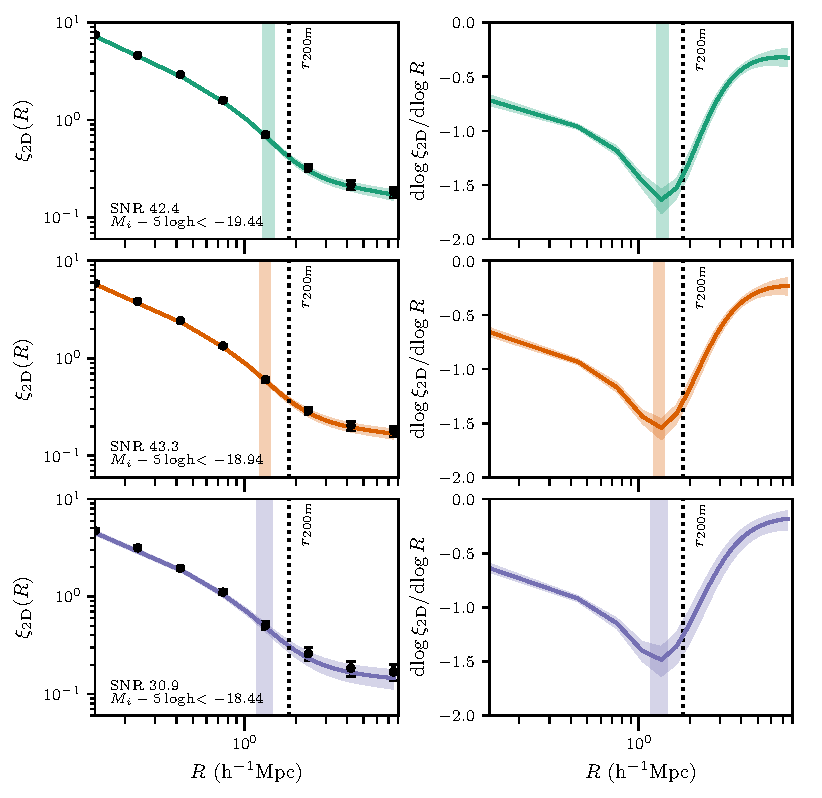
\includegraphics[scale=0.65]{2D_graphs.pdf}
\caption{The estimates of the two-dimensional cross-correlation
signals (black dots) are shown in the left column. The colored
curves show the two-dimensional model fits of the functional
form in Equation~\ref{eq:surface}. The magnitude limit applied to the galaxy
catalog is indicated in each row along with the signal-to-noise ratio (SNR). 
The vertical, shaded regions indicate the estimates of the locations of 
steepest slope of the profiles as estimated from the corresponding minima of the
derivative profiles, which are shown in the right column. For
comparison, the location of the $r_{\mathrm{200m}}$ radius as
calculated from the average cluster sample properties is indicated
by the black, dotted lines.}
   \label{fig:2D_graphs}
\end{figure}

\begin{figure}
    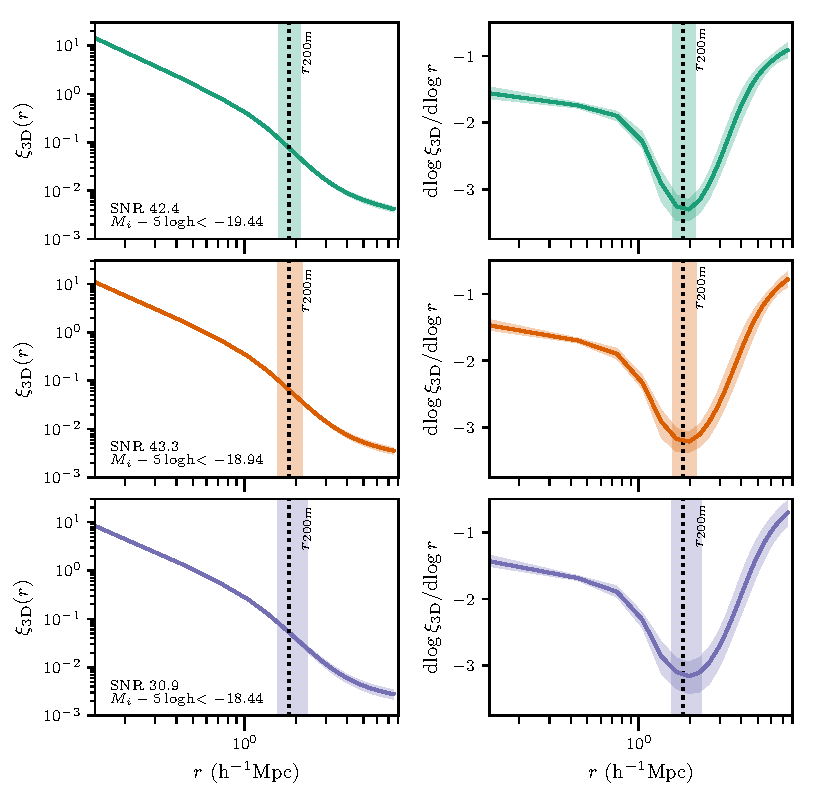
\includegraphics[scale=0.65]{3D_graphs.pdf}
\caption{The estimates of the three-dimensional cross-correlation
signals are shown in the left column. The colored curves show the
model fits of the functional form in Equation~\ref{eq:model}. The magnitude
limit applied on the galaxy catalog is indicated in each row along with 
the signal-to-noise ratio (SNR). The vertical, shaded regions indicate the 
estimates of the splashback radii as estimated from the corresponding minima 
of the derivative profiles, which are shown in the right column. For comparison, 
the location of the $r_{\mathrm{200m}}$ radius as calculated from the
average cluster sample properties is indicated by the black, dotted
lines.}
   \label{fig:3D_graphs} 
\end{figure}


\begin{table}
    \centering
    \caption{We list the signal to noise ratios (SNRs) of our
different estimates of the two-dimensional cross-correlation
obtained by using the different galaxy samples. For comparison: The SNR
achieved by \citet{more2016detection} is 263.0. It is much higher
due to size of the cluster sample used in their study.}
    \label{tab:snr}
    \begin{tabular}{cccc}
    \hline
    %clu & PSZ2 & PSZ2 & PSZ2 & PSZ2 & PSZ2 & PSZ2 & MCXC & MCXC & MCXC\\  
    %\hline 
    gal cat & PS 21 & PS 21.5 & PS 22 \\ 
    \hline
    \hline
   SNR & 42.4 & 43.3 & 30.9 \\%& 16.5 & 17.5 & 13.3 & & &\\ 
    \hline
    \end{tabular} 
\end{table}

\begin{table*}
    \centering
    \caption{We list our findings for the fitting parameters obtained from cross-correlating the galaxy cluster sample with the different galaxy catalogs. For each parameter estimate the median as well as the 16\% and 84\% quantiles of the posterior distribution are given. We also list the estimated locations of the steepening feature in the two-dimensional cross-correlation signal ($R_{\mathrm{sp}}^{\mathrm{2D}}$) as well as the three-dimensional splashback radius ($r_{\mathrm{sp}}^{\mathrm{3D}}$). In the last column the minimal, reduced $\chi^2$ value of the model fit is indicated. The two-dimensional posterior distributions of the fitting parameters are displayed in 
Figure~\ref{fig:corner_21} up to Figure~\ref{fig:cornerblue}.}
    \label{tab:fit_parameters}
    \begin{tabular}{cccccccccccccc}
    \hline 
gal cat & $\log_{10}(\rho_{\mathrm{s}})$ & $\log_{10}(\alpha)$ & $\log_{10}(r_{\mathrm{s}})$ & $\rho_{\mathrm{0}}\cdot 10^{5}$ & $s_{\mathrm{e}}$ & $\log_{10}(r_{\mathrm{t}})$ & $\log_{10}(\beta)$ & $\log_{10}(\gamma)$ & $R_{\mathrm{sp}}^{\mathrm{2D}}$ & $r_{\mathrm{sp}}^{\mathrm{3D}}$ & $\chi^2/\nu$ \\
\hline 
\hline 
PS 21 & $-2.93_{-0.50}^{+0.44}$ & $-1.06_{-0.18}^{+0.14}$ & $0.35_{-0.24}^{+0.27}$ & $17.9_{-8.6}^{+7.5}$ & $0.78_{-0.19}^{+0.24}$ & $0.123_{-0.122}^{+0.051}$ & $0.74_{-0.31}^{+0.21}$ & $0.35_{-0.21}^{+0.13}$ & $1.384_{-0.096}^{+0.088}$ & $1.86_{-0.26}^{+0.25}$ & $1.524$ \\
\hline
PS 21.5 & $-2.93_{-0.45}^{+0.45}$ & $-0.95_{-0.16}^{+0.13}$ & $0.32_{-0.25}^{+0.25}$ & $10.3_{-6.5}^{+4.7}$ & $0.56_{-0.22}^{+0.25}$ & $0.095_{-0.115}^{+0.045}$ & $0.74_{-0.32}^{+0.24}$ & $0.27_{-0.19}^{+0.12}$ & $1.323_{-0.086}^{+0.080}$ & $1.85_{-0.30}^{+0.26}$ & $0.285$ \\
\hline
PS 22 & $-2.95_{-0.44}^{+0.49}$ & $-0.91_{-0.17}^{+0.14}$ & $0.28_{-0.27}^{+0.25}$ & $6.2_{-5.1}^{+2.8}$ & $0.41_{-0.28}^{+0.25}$ & $0.094_{-0.190}^{+0.060}$ & $0.76_{-0.36}^{+0.29}$ & $0.24_{-0.27}^{+0.14}$ & $1.31_{-0.14}^{+0.11}$ & $1.90_{-0.40}^{+0.32}$ & $0.211$ \\
\hline
PS 21.5(R) & $-2.17_{-0.58}^{+0.86}$ & $-1.03_{-0.33}^{+0.33}$ & $-0.02_{-0.46}^{+0.31}$ & $8.3_{-8.8}^{+4.4}$ & $0.59_{-0.37}^{+0.34}$ & $0.09_{-0.32}^{+0.13}$ & $0.53_{-0.32}^{+0.23}$ & $0.27_{-0.32}^{+0.20}$ & $1.22_{-0.10}^{+0.12}$ & $1.94_{-0.34}^{+0.32}$ & $1.361$ \\
\hline
PS 21.5(B) & $-2.90_{-0.38}^{+0.38}$ & $-0.64_{-0.14}^{+0.12}$ & $0.34_{-0.24}^{+0.24}$ & $12.7_{-6.5}^{+5.5}$ & $0.61_{-0.18}^{+0.23}$ & $0.26_{-0.20}^{+0.13}$ & $0.48_{-0.16}^{+0.12}$ & $0.44_{-0.30}^{+0.23}$ & $1.505_{-0.089}^{+0.091}$ & $2.29_{-0.20}^{+0.19}$ & $1.132$ \\
\hline
    \end{tabular} 
\end{table*}

\begin{figure*}
\centering{
  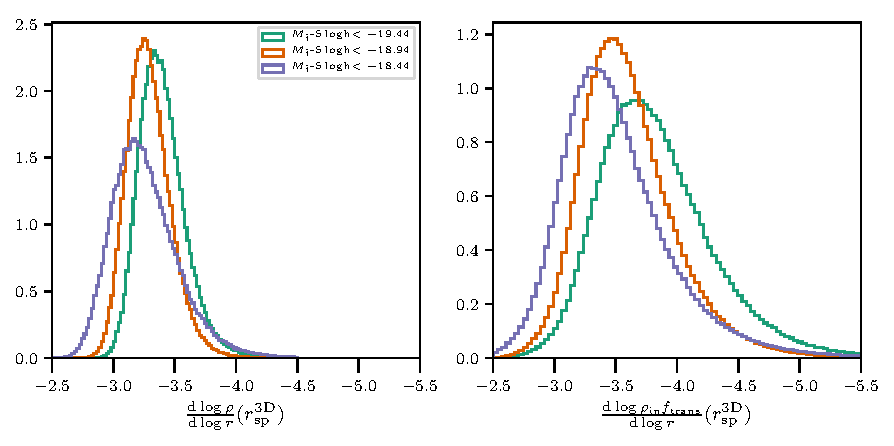
\includegraphics[scale=0.8]{derivatives.pdf}}
\caption{We show the distributions of the logarithmic derivatives of
the three-dimensional cross-correlation signals at the location of
the splashback radius. In the left panel the distributions of the
derivatives of the full profiles are shown, whereas only the inner
halo term (namely $\rho_{\mathrm{in}}f_{\mathrm{trans}}$) is
considered in the right panel.}
   \label{fig:derivatives} 
\end{figure*}
\begin{figure*}
\centering{
    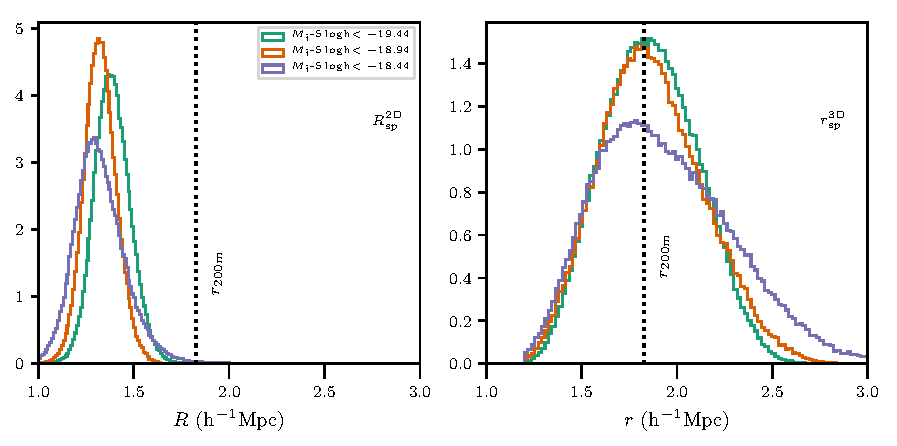
\includegraphics[scale=0.8]{splashback.pdf}}
\caption{Shown are the posterior distributions of the inferred
locations of steepest slope of the two- and three dimensional
cross-correlation signals. On the left side the distributions of the
locations of the two-dimensional steepening feature
($R_{\mathrm{sp}}^{\mathrm{2D}}$) are shown, whereas the
distributions of the three-dimensional counterparts
($r_{\mathrm{sp}}^{\mathrm{3D}}$) are shown on the right. The
magnitude limit applied to the galaxy catalogs is indicated for each
distribution. Note that the colors of the distributions match with
the colors used in Figure~\ref{fig:2D_graphs} and
Figure~\ref{fig:3D_graphs}. For comparison, the location of the virial
radius $r_{\mathrm{200m}}$ as calculated from the average cluster
sample properties is indicated by the black, dotted lines.}
   \label{fig:splashback} 
\end{figure*}
\begin{figure}
    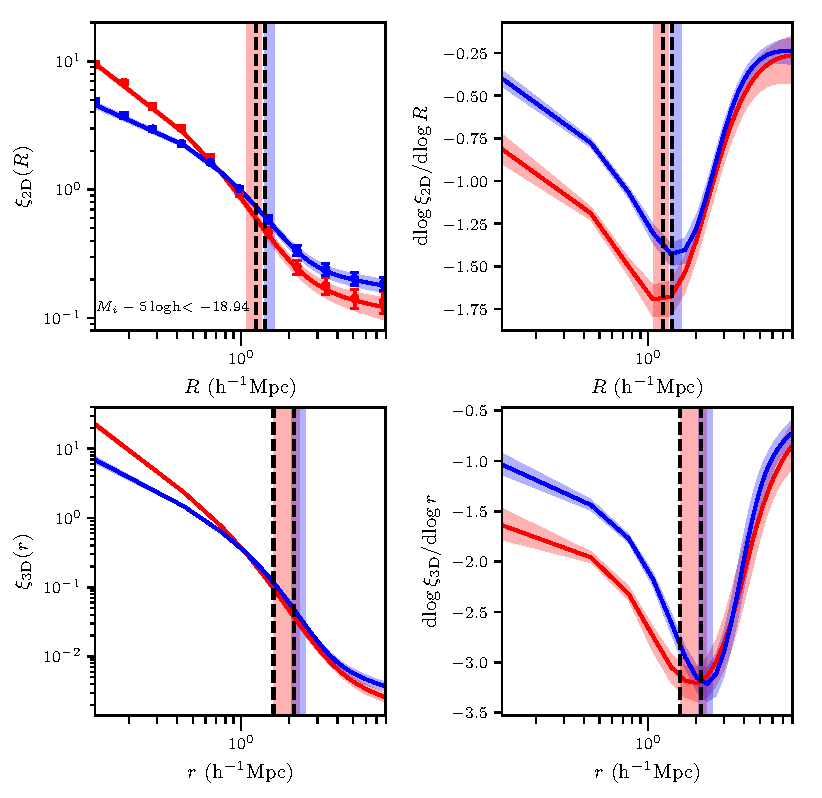
\includegraphics[scale=0.65]{color_separated.pdf}
\caption{\textit{Top row: } The two-dimensional cross-correlations
of the red and blue galaxy populations as inferred by
cross-correlating the cluster sample with the color-separated
subsamples that were extracted from the PS 21.5 galaxy catalog are
shown in the left panel, whereas the associated derivative profiles
are shown on the right. The vertical, shaded bands indicate the
locations of steepest slope of the cross-correlation signal as
inferred from the two subsamples, whereas the black, dashed lines
indicate the upper and lower bounds of the same feature but as
estimated from the full PS 21.5 galaxy catalog. \textit{Bottom row:
} We show the three-dimensional cross-correlations as
inferred by cross-correlating the cluster sample with the
color-separated galaxy subsamples, as well as the corresponding
splashback radii (indicated by the colored, vertical bands) and
their derivative profiles. Here, the black, dashed lines indicate
upper and lower bounds of the three-dimensional splashback radius
corresponding to the full PS 21.5 galaxy sample.}
   \label{fig:color_curve} 
\end{figure}

\begin{figure}
    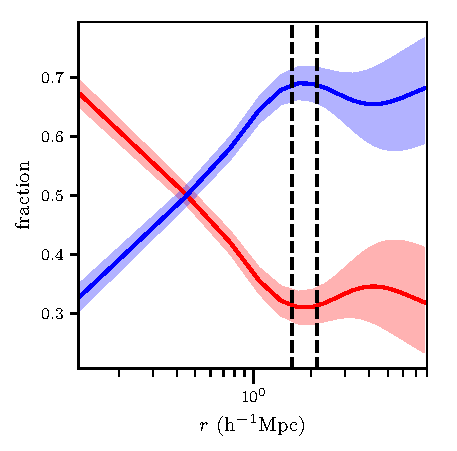
\includegraphics[width= \columnwidth]{color_fraction.pdf}
\caption{Fractional contributions of the red and blue galaxy
populations to the total galaxy number density. We show the
locations of the splashback radii associated with the two subsamples
with the colored, vertical bands and the upper and lower bounds of
the splashback radius obtained from the full PS 21.5 catalog with
the black, dashed lines.}
   \label{fig:color_fraction} 
\end{figure}
The right panels in Figure~\ref{fig:2D_graphs} show the
corresponding analytical derivatives of the two-dimensional
cross-correlations and the 68\% confidence interval based on our
model fits. The logarithmic derivatives show a distinct steepening
feature at around $1.3-1.5~\mpch$. The figure shows that the
location of the steepest slope does not change appreciably when the
magnitude limit is changed, even though we use a sample which is one
magnitude deeper than $M_{\rm i}-5\log h=-19.44$. The 68\%
confidence interval of the location of the steepest slope is
indicated by the vertical, shaded region. We also show the location
of the virial radius $r_{\mathrm{200m}}$ based on the Planck SZ mass estimate 
as a black, dotted line in each panel.

We use the posterior distributions of our model parameters to infer
the three-dimensional cross-correlation and its logarithmic
derivative. These inferences along with the corresponding 68\%
confidence intervals are presented in Figure~\ref{fig:3D_graphs},
maintaining the same color scheme as in Figure~\ref{fig:2D_graphs}
for ease of comparison. The three-dimensional cross-correlations
also show significant steepening in each of the cases that we have
explored, reaching logarithmic derivatives steeper than $-3$. The
inferred 68\% confidence regions for the locations of the steepest
slope of the three-dimensional cross-correlations are shown with
vertical, shaded regions in each panel. The posterior
distributions of the locations of the steepest slope in the
two-dimensional and three-dimensional cross-correlations can be
found in the left hand and the right hand panels of
Figure~\ref{fig:splashback}, respectively. The estimates of the splashback radii
for each of the samples are listed in Table~\ref{tab:fit_parameters}
and our results show that the location of the splashback radius does
not depend upon the sample once we use galaxies fainter than $M_{\rm
i}-5\log h=-19.44$. Our measurements have an accuracy of $\sim$15\%.

Following \citet{baxter2017halo}, we also present the values of the
logarithmic derivatives at the location of the steepest slope for
the total three-dimensional cross-correlations, as well as those for
the inner halo term in the left and right hand panels of
Figure~\ref{fig:derivatives}, respectively. The logarithmic slope of the 
cross-correlation is significantly steeper than $-3$ at the location 
of the splashback radius, making it difficult to
be reproduced by classical fitting functions like the NFW profile,
which reach such slopes only asymptotically and even that only
without the presence of the outer 2-halo term. This provides
evidence for the existence of the splashback feature.

We perform a preliminary comparison of the measurements with
expectations from cold dark matter models. The average halo mass of
the PSZ2 clusters as estimated from the Sunyaev-Zeldovich signal
is $M_{\rm 500c}=3.0\times10^{14}$ $\msunh$. We convert this mass
estimate to $M_{\rm 200m}=6.2\times10^{14}$ $\msunh$ using the average
concentration mass relation of halos following
\citet{HuKravtsov:2003}. Given the average mass and redshift of our
cluster sample, we calculate the expected splashback radius to be
$1.89$ $\mpch$. We base this estimate on the fitting functions
presented in \citet{more2015splashback}. The splashback radius we
find for the three samples is consistent with this expectation,
although we can not rule out $15\%$ deviations in either directions,
given our large error bars.

%\subsection{Location of the Splashback radius}
%Using the estimates of the fitting parameters obtained from the MCMC procedure the posterior distributions of the locations of the splashback radii as inferred from the different datasets are obtained. The distributions are shown in Figure~\ref{fig:splashback}, where the panel on the left displays the posterior distribution of the projected splashback radius ($R_{\mathrm{sp}}^{\mathrm{2D}}$) and the right panel the distributions of the three dimensional, physical counterparts ($r_{\mathrm{sp}}^{\mathrm{3D}}$). %The top row shows the results as inferred by using the DP estimator whereas the LS estimator was used in the lower panels. 
%The survey depth is indicated for each distribution and the colors correspond to the colors already used in Figure~\ref{fig:2D_graphs} and Figure~\ref{fig:3D_graphs}. The estimates of the splashback radii are listed in Table~\ref{tab:splashbacks}. 
%We notice a weak anti-correlation between survey depth and the location of $R_{\mathrm{sp}}^{\mathrm{2D}}$. However, the trend is no longer visible in the posterior distributions for $r_{\mathrm{sp}}^{\mathrm{3D}}$.

Next we present our measurements of the projected and
three-dimensional cross-correlations of red and blue galaxies
satisfying $M_{i}-5\log h<-18.94$ with our SZ-selected cluster
sample in the top and bottom left hand panels of
Figure~\ref{fig:color_curve}, respectively. The shaded regions show
the 68\% confidence intervals from our fits. The vertical, shaded
bands with different colors indicate the 68\% confidence regions of
the locations of the steepest slope of the two- and the
three-dimensional cross-correlations. The black dashed lines show
these ranges for the entire galaxy sample without regard to color.
The best fit parameters as well as the inferred splashback radii are
listed in Table~\ref{tab:fit_parameters}. The right hand
panels show the corresponding inferred logarithmic derivatives. We
see that the red galaxies have a steeper cross-correlation profile
than the blue galaxies. Although there is a tendency for the red
galaxies to have a smaller splashback radius, the differences we see
are not statistically significant given the current errors. The
slopes of the three-dimensional cross-correlations reach values
steeper than -3 at the splashback radius.

Nevertheless, the fact that we detect the splashback radius for blue
galaxies is significant. The implication of this result is that
there needs to be a reasonable fraction of blue galaxies that fall
into the cluster and continue to stay blue even after reaching their
apocenters. Star forming galaxies in models which quench their star
formation on a timescale shorter than the orbital time scale, are
not expected to show the presence of the splashback radius. A
quantitative exploration of the implications is beyond the scope of
this work, but will be followed up in the future.

In Figure~\ref{fig:color_fraction}, we show the fractional
contributions of the red and blue galaxies to the total,
three-dimensional cross-correlation \footnote{The fractions are
obtained by performing an appropriate number density weighting.}.
The red galaxies dominate the central parts of the galaxy clusters
but become sub-dominant as we move further away from the centers of the 
clusters. We see a sharp increase of the fractional contribution of
red galaxies below the splashback radius. On scales larger than the
splashback radius, the populations are consistent with a constant
fraction of $\approx 70\%$ blue and $\approx 30\%$ red galaxies.
%\subsection{Deprojection}
%In Figure~\ref{fig:deprojection} the estimate of the three dimensional density profile as obtained from the alternative deprojection algorithm described in Section~\ref{sec:Deprojection} is presented. The deprojection method was exploited for the PS 21.5 catalog. The density profile obtained by the standard MCMC fitting procedure outlined above is added to the data-points for better comparison. One can observe that the deprojection algorithm manages to reproduce the density profile obtained by the standard procedure very well on scales below 2 h$^{-1}$ Mpc but experiences an overshoot on larger scales.



%\begin{figure}
%   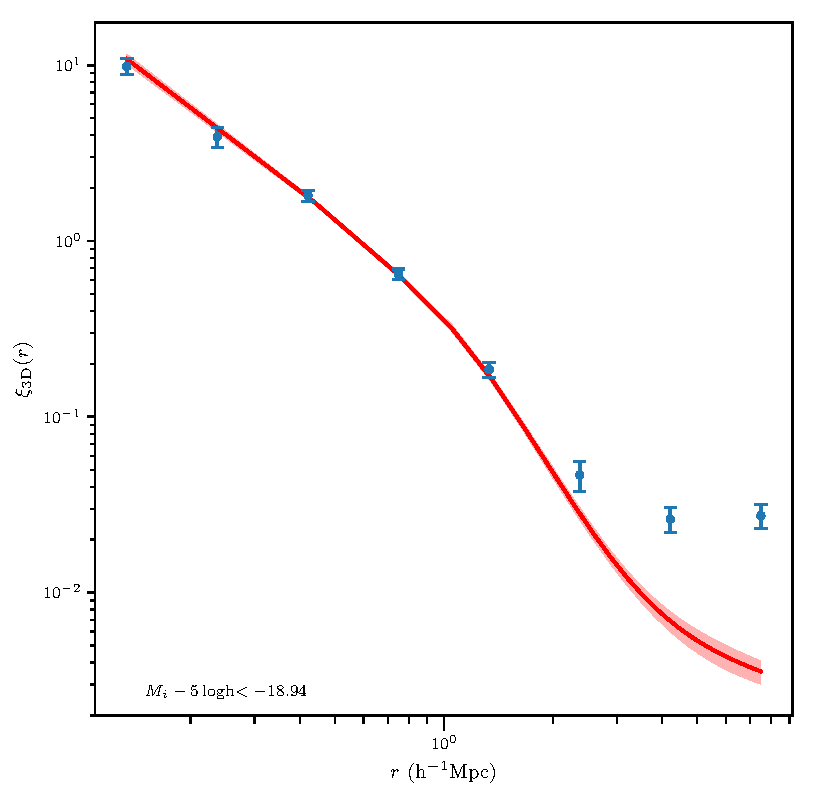
\includegraphics[width= \columnwidth]{deprojection.pdf}
%\caption{The data-points indicate the estimate of the three dimensional density profile as inferred by using the deprojection algorithm outlined in Section~\ref{sec:Deprojection} on the PS 21.5 galaxy sample. Additionally, the density profile obtained by exploiting the PS 21.5 galaxy catalog and the standard MCMC fitting procedure are shown for comparison.}
%   \label{fig:deprojection} 
%\end{figure}
%\newpage

\section{Future work}
\label{sec:Future}

%Further, by comparison of the estimates of the splashback radius listed in Table~\ref{tab:splashbacks} with the expectation of $1.89 $ h$^{-1}$ Mpc for the three dimensional, physical splashback radius $r_{\mathrm{sp}}^{\mathrm{3D}}$ we can conclude that our results are in agreement with the theoretical prediction. On the contrary, we can not confirm the discrepancy between the theoretical and observed location of the splashback radius that was found by \citet{more2016detection} when correlating optically selected clusters with SDSS galaxies.

%From the comparison in Figure~\ref{fig:3D_graphs} we can conclude that the choice of the depth of the catalog does not alter the shapes of the density profiles significantly nor does it change the location of the splashback radius in a systematic manner. 

% Move into future work section:
As it can be seen from Table~\ref{tab:snr}, the signal-to-noise
ratio of our measurement is lower when using the PS 22 catalog
compared to the other two estimates. This has two causes: Firstly,
the sky-coverage of the PS 22 catalog is $\approx$ 25\% lower than
for PS 21 and PS 21.5 since more regions had to be excluded due to
the survey depth being too low in those regions. Therefore, some
clusters from the PSZ2 catalog are missed when the PS 22 catalog is
exploited, which reduces the statistics. Secondly, as we consider
fainter galaxies, the contamination from background galaxies is
increased. This requires a better estimate of the uncorrelated
background component. A more precise estimation of the uncorrelated
background contamination would be possible by using a random galaxy
catalog in addition to the random cluster sample. This would allow
to use the more sophisticated Landy \& Szalay estimator
\citep{landy1993bias} to perform the background subtraction.
% (see Section~\ref{sec:est_surf_den}). 

Another approach to increase the statistics of the measurements would be to increase the redshift range in which clusters are being considered. We chose $0.03 \leq z \leq 0.33$ in order to keep the analysis comparable to \citet{more2016detection}. However, this cut reduces the cluster sample size. Increasing the redshift range has its own limitations, though. It would be required to use a brighter magnitude limit for galaxies, which reduces the number of galaxies that can be used to infer the cross-correlation signal. This results in a trade-off and we could investigate the optimal redshift range. Alternatively, other cluster samples that do not rely on optical cluster finding such as Xray based surveys might serve as independent and larger cluster samples. 
%We are considering to use the meta-catalog of X-ray detected clusters of galaxies (MCXC) which combines sevaral X-Ray based cluster catalogs for further investigations. The catalog is based on the ROSAT All-Sky survey \citep{voges1999rosat}. 
Another plausible approach would be to consider a smaller region of
the sky, meaning also less clusters but with a deeper field of view,
such as in the case of the Hyper Suprime-Cam at Subaru Telescope,
which will survey $\approx 1400$ deg$^2$ of the sky and achieve a
depth of 26.2 magnitudes \citep{takada2010subaru}.


%We present the result of our attempt to deproject the surface density profile in Figure~\ref{fig:deprojection}. We achieve good agreement between the standard and the deprojection procedure on scales below $2$ h$^{-1}$ Mpc but record a significant disagreement on larger scales. Therefore, we conclude that the general procedure is working but requires improvement. We suspect that including effects from masking and survey boundaries into the deprojection algorithm could improve the agreement. The procedure to do so is outlined in Section~\ref{sec:deprojection_math} but was not implemented so far. 

% I do not agree with this paragraph. I will tell you why later on.
%From Figure~\ref{fig:color_fraction} we can confirm that the splashback feature is strongly associated with a sharp increase in the red fraction as it was observed by \citet{baxter2017halo} before. On the contrary, \citet{baxter2017halo} find that the density profile of the blue population reaches a constant logarithmic derivative of -1.5 at large radii outside of the splashbak radius, as it would be expected for purely in-falling material. This is not reproduced in our study where the density profile of the blue population flattens out further and reaches logarithmic derivatives below -1. We propose that this deviation from a purely in-falling population of galaxies might be caused by group preprocessing: preprocessing referrs to a situation where a galaxy is in-falling onto a large halo but has been acrreated onto a smaller subhalo before which itself is being accreated onto the larger halo at the time of observation. In such a scenario, the galaxy seems to be on its first in-fall but has actually passed through the central part of a smaller subhalo before \citep{fujita2004pre}. Therefore, the quenching of the galaxy started earlier and it might have already changed to a red sequence galaxy before reaching the splashback radius of the large halo. It was found by \citet{wetzel2013galaxy} that such galaxies make up for at least 30\% of the quiescent galaxies in a cluster which can increase to over 50\% for massive clusters above $10^{14} M_{\sun}$. Since mainly massive clusters are studied in this work we expect a large contribution from preprocessed galaxies which could explain the discrepancy from \citet{baxter2017halo}. We note that our investigations on the distributions of the blue and red subpopulations are far from complete. A thorough study would have to take into account the different masses and velocities of the individual galaxies in order to get a more precise picture. We note as well that we used a very simple, idealistic way to separate the galaxy catalog in subsamples relying on only two photometric bands and that a considering more bands might improve the results.

% Already included before.
%Although, we find good agreement with the theory it would be premature to jump to conclusions about the nature of the splashback radius from this study. Due to the small cluster sample used in this work we achieve much lower statistic than \citet{more2016detection}. As evident from Table~\ref{tab:splashbacks} our estimates of the splashback radii suffer from relative errors of $\approx$ 15\%. 

In our work, we have assumed that the brightest central galaxy
resides at rest with respect to the center of the dark matter halo.
The mass dependence of the exact mis-centering fractions are not
well understood \citep{Skibba:2011, Hoshino:2015}.
\citet{baxter2017halo} have shown that mis-centering effects could
in principle decrease the significance of the evidence for the
splashback radius, but do not affect the location of the splashback
radius, significantly. Nevertheless we plan to pursue models
including mis-centering to fit to our measurements.

%Apart, from statistical errors there are also multiple systematic sources of errors that have to be investigated more thoroughly before we can draw any definitive conclusions from our results: Although, the central cluster positions have been adjusted manually it can not be guaranteed that the corrected positions are at the actual centers of the clusters. Firstly, the visual inspection is prone to human error of course and secondly it is assumed that the gravitational center of the cluster lays at the same position as the brightest central galaxy, which might not be true in general. The effect of such misplacements might be investigated by artificially displace some subsample of the clusters and study the influence on the location of the splashback radius. 

% This is irrelevant because the stars are not correlated with the galaxy clusters, so should drop out.
%Regarding the galaxy catalog, the exploited star-galaxy separation is of very simplistic nature and the extracted catalog might still suffer from contaminations from stars. It might be worth to consider a more sophisticated separation method.

% This is very commonly known, so not necessary to be stated.
%Some tests outlined in Section~\ref{sec:convergence} have been exploited to investigate the mixing behavior and convergence of the MCMC chains used in the fitting procedure as described in Section~\ref{sec:MCMC}. However, it has to be noted that there is no mathematical tool available, that can confirm the convergence of MCMC chains without fail. Therefore, although the performed tests suggest that the chains are convergent we can not exclude that they may have not reached a static distribution. 

Lastly, but most importantly, the investigation of any systematics
which might originate from the SZ selection of the Planck clusters
is beyond the scope of the current work. We caution that there may
be residual systematics in the selection which could affect the
interpretation of our measurements. We will investigate such
selection systematics with the help of hydrodynamical simulations.

\section{Conclusions}
\label{sec:Conclusions}
The splashback radius of dark matter halos is a unique observational
probe of the mass accretion rate of dark matter halos. Although the
splashback radius has been well-characterized in simulations, the
observational evidence for the splashback radius presented using
optical cluster catalogs has come under intense scrutiny. In this
work, we tackle this issue by searching for evidence of the
splashback radius in galaxy clusters found by the Planck surveyor using
the thermal Sunyaev-Zeldovich effect. The use of this sample avoids
the circularity of using photometric galaxy catalogs to identify
clusters as well as to detect the splashback radius. 

%By using an independent cluster sample that was not obtained by optical cluster finding, we manage to observe the splashback radius at the expected location. 

We cross-correlate these clusters with photometric galaxies from the
Pan-STARRS survey to obtain the two-dimensional cross-correlation
function and search for evidence for the splashback feature.
Additionally, we divided our galaxy catalog into two subsamples of
red and blue galaxies and investigated the cross-correlations of the
two subsamples with the clusters, separately.

%Subsequently, we searched for the signature of the splashback feature in the cross-correlation signals. We also separated the extracted galaxy catalog on color into a subsample of red and one of blue galaxies and studied their radial distributions in the halos. 

Our main findings can be summarized as follows:
\begin{itemize}
\item We detect a clear signature of a steepening feature in the
cross-correlation of Planck SZ clusters with Pan-STARRS
galaxies. The steepest logarithmic slopes that we find in our cross-correlation
signals are steeper than $-3$, and would hence be poorly fit by the
NFW profile. We associate this feature with the splashback feature.
\item The location of the inferred splashback radius is $r_{\rm
sp}=1.85_{-0.30}^{+0.26}$ $\mpch$, which is consistent with expectations
from numerical simulations for
halos of an average mass $M_{\rm 500c}=3.0\times10^{14}\msunh$ at an
average redshift of $z=0.18$ in a collision-less dark matter Universe. 
However, given the errors we cannot
currently rule out $\sim15\%$ deviations from these expectations.
\item We find that the location of the steepest slope does not
strongly depend on the magnitude of the galaxy samples we use, once
we go fainter than $M_i-5\log h=-19.44$.
% Explore dynamical friction effects by going even two magnitudes brighter later.
%Hence, we conclude that the discrepancy found by \citet{more2016detection} is caused by systematics originating from the optical cluster finding algorithm
\item By separately studying the cross-correlation of red and blue
galaxies with the clusters, we present evidence for the presence of
the splashback feature in both populations. This implies that the
star formation of a sizable number of blue galaxies does not get
quenched during their first orbit through the halo.
\item We also detect a sharp increase in the fraction of red
galaxies associated with the splashback radius. 
%clear correlation between the location of the splashback feature and an associated sharp increase in the red fraction. Further, we record indications pointing towards the group preprocessing scenario.
% \item We made a first attempt to deproject the two dimensional correlation signal. We find good agreement between the deprojected signal and the three dimensional profile obtained from the standard algorithm on scales up to 2 h$^{-1}$ Mpc, from which we conclude that the method works, basically. However, we note a strong disagreement on larger scales, which we suspect to originate from the missing correction for masking and survey border effects.
\end{itemize}

Our curated galaxy catalogs from the Pan-STARRS survey for different
depths and the corresponding masks are available and can be send
upon request.


%As it is noted in Section~\ref{sec:Discussion} there is still need for further investigation and improvement. We plan on utilizing the meta-catalog of X-ray detected clusters of galaxies (MCXC) which is based on the ROSAT All-Sky survey \citep{voges1999rosat} as yet another independent cluster sample. Also, the systematic biases stemming from the selection of clusters through the Sunyaev-Zeldovich effect have to be clarified. To that goal, performing hydrodynamic simulations might have to be considered. Further, the use of random galaxies would improve the estimation of the uncorrelated background component and increase the sensitivity espicially when using faint galaxies. Interesting results regarding the formation history of galaxies in clusters were found. However, the correct interpretation of those results requires further, more detailed studies. Having obtained a very good agreement between the deprojection algorithm and the standard procedure exploited we are confident that the remaining discrepancy can be diminished by further improvement of the algorithm, such as accounting for masking and survey boundaries.

\section*{Acknowledgements}
DZ is grateful to Kavli IPMU for its hospitality during this
research project. SM is supported by a grant-in-aid by the Japan
Society for Promotion of Science (JSPS), grant number 16H01089.
The Pan-STARRS1 Surveys (PS1) and the PS1 public science archive
have been made possible through contributions by the Institute for
Astronomy, the University of Hawaii, the Pan-STARRS Project Office,
the Max-Planck Society and its participating institutes, the Max
Planck Institute for Astronomy, Heidelberg and the Max Planck
Institute for Extraterrestrial Physics, Garching, The Johns Hopkins
University, Durham University, the University of Edinburgh, the
Queen's University Belfast, the Harvard-Smithsonian Center for
Astrophysics, the Las Cumbres Observatory Global Telescope Network
Incorporated, the National Central University of Taiwan, the Space
Telescope Science Institute, the National Aeronautics and Space
Administration under Grant No. NNX08AR22G issued through the
Planetary Science Division of the NASA Science Mission Directorate,
the National Science Foundation Grant No. AST-1238877, the
University of Maryland, Eotvos Lorand University (ELTE), the Los
Alamos National Laboratory, and the Gordon and Betty Moore
Foundation.

Based on observations obtained with Planck
(http://www.esa.int/Planck), an ESA science mission with instruments
and contributions directly funded by ESA Member States, NASA, and
Canada.  Some of the results in this paper have been derived using
the HEALPix (K.M. Górski et al., 2005, ApJ, 622, p759) package

\bibliographystyle{mnras}
\bibliography{RSP_library} 



\appendix

\section{Sky maps}
\label{sec:figures}
We present the sky locations of the SZ selected clusters from the PSZ2
catalog that were used in our study in Figure~\ref{fig:planck_fig}.
The purple areas mark the masked out regions as defined by the union
selection function of the PSZ2 catalog. The sky maps in
Figure~\ref{fig:heal_map} show the survey masks of our three galaxy
catalogs. All sky maps presented in this section use the ICRS
coordinate system.

\begin{figure}
\centering{
    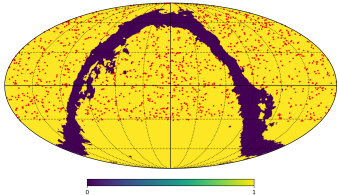
\includegraphics[scale=0.8]{Planck_pres.png}}
\caption{Sky map showing the sky positions of the used clusters as
selected from the PSZ2 catalog. In total 596 clusters have been
selected. The purple areas mark the regions that are excluded by the
union survey selection function. Note that all clusters with
$\delta<-31\degr$ have been removed since this region is not covered
by the Pan-STARRS 3$\pi$ Steradian survey. The ICRS coordinate
system is used.}
    \label{fig:planck_fig} 
\end{figure}

\begin{figure*}
    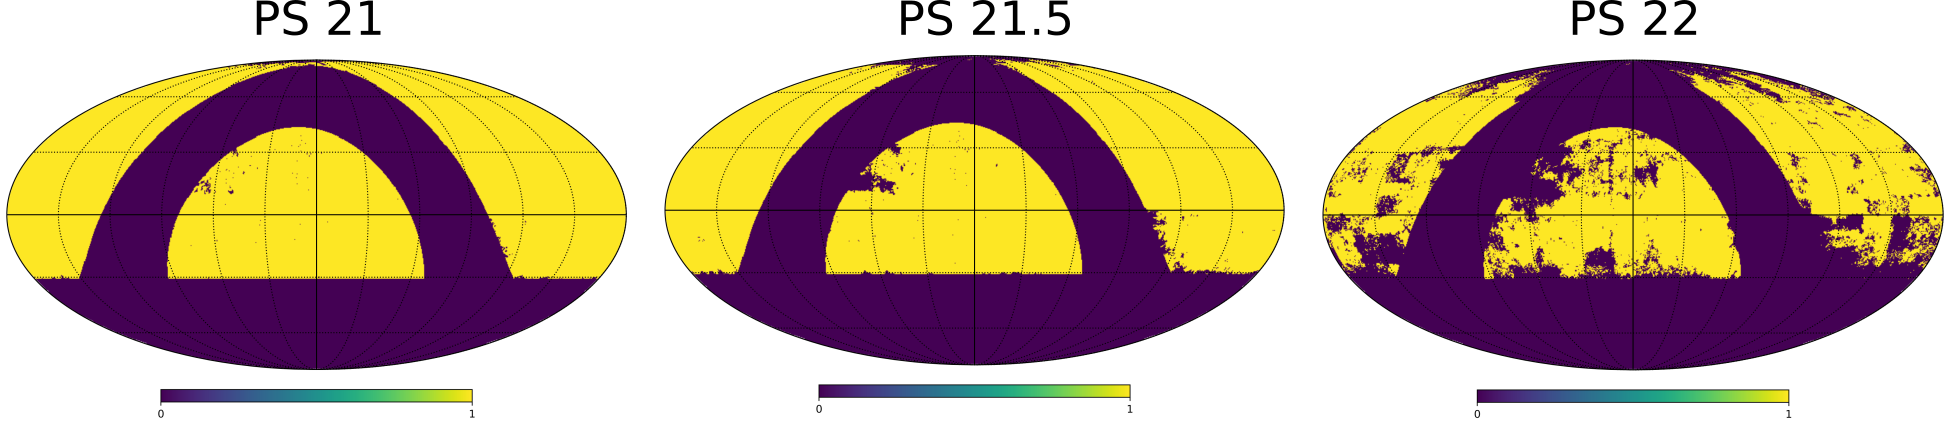
\includegraphics[width= \textwidth]{heal_maps.png}
\caption{Sky maps displaying the masked out regions of the used
galaxy catalogs extracted from the Pan-STARRS 3$\pi$ Steradian
survey in purple. The ICRS coordinate system is used.}
   \label{fig:heal_map} 
\end{figure*}

%\section{Convergence of MCMC chains
%\label{sec:convergence}
%Three different methods are exploited in order to assess the convergence of the MCMC chains. Firstly, the general behavior of the chains is monitored and it is checked that they are well behaved, meaning that they converge to a common point in the parameter space, at least visually. With the same goal in mind the autocorrelations of the chains are calculated and it is assured that the autocorrelations are monotonically decreasing as the chains grow.

%The second method involves performing a statistical test, named after Geweke \citet{geweke1991evaluating} which relies on methods from spectral analysis to address the issues of biases and variance alike. Imagine attempting to estimate the mean of a function $f$ which depends on the simulated parameter $\theta$. After $n$ iterations of the chain the estimate of the mean becomes
%\begin{equation}
%\bar{f}_n=\frac{\sum_{i=1}^n f(\theta^{(i)})}{n}
%\end{equation}
%and Geweke states that the asymptotic variance of that estimator yields $S^G(0)/n$, where $S^G(0)$ indicates the spectral density at frequency 0. The Geweke statistic is calculated by using two subsamples of the simulated parameter set. Geweke suggests taking the first 10\% of the iterations as the first sample $n_{\mathrm{A}}$ and the last 50\% of the iterations to be the second sample $n_{\mathrm{B}}$. Note that $n_{\mathrm{A}}/n + n_{\mathrm{B}}/n < 1$ to assure asymptotic independence of the two parts of the chain. For both subsets the estimate of the mean is calculated yielding $\bar{f}(\theta)_{\mathrm{A}}$ and $\bar{f}(\theta)_{\mathrm{B}}$, respectively. Further, the corresponding asymptotic variances are calculated as well to obtain $S^G_{\mathrm{A}}(0)/n_{\mathrm{A}}$ and $S^G_{\mathrm{B}}(0)/n_{\mathrm{B}}$, respectively. Geweke's convergence diagnostic is than constructed as
%\begin{equation}
%Z_{\mathrm{(A,B)}}=\frac{\bar{f}(\theta)_{\mathrm{A}}-\bar{f}(\theta)_{\mathrm{B}}}{n_{\mathrm{A}}^{-1}S^G_{\mathrm{A}}(0)-n_{\mathrm{B}}^{-1}S^G_{\mathrm{B}}(0)},
%\end{equation}
%which approaches a standard normal distribution according to the central limit theorem if the samples are being drawn from a stationary distribution. Geweke argues that the convergence statistic may be used to determine how many of the initial steps must be regarded as burn-in steps and therefore must be disregarded \citet{cowles1996markov}.

%Lastly, the Heidelberger and Welch test is performed \citep{heidelberger1983simulation}. The test combines approaches from spectral analysis with a convergence test by \citet{schruben1983optimal} designed to detect non-stationarity in a simulated set of parameters. Denoting the jth simulated parameter value in the chain as $\theta_j$ and the total number of iterations in the chain as $n$ the statistic $B_n(t)$ is calculated as
%\begin{equation}
%B_n(t)=\frac{T_{[nt]}-[nt]\bar{\theta}}{\sqrt{nS(0)}} , 0 \leq t \leq 1
%\end{equation}
%where $[.]$ indicates the floor function and
%\begin{align}
%T_k=\sum_{j=1}^k \theta_j \\
%\bar{\theta}=\frac{\sum_{j=1}^n \theta_j}{n}
%\end{align}
%and $S(0)$ indicates the spectral density at frequency 0 once again. The claim is that if convergence of the chain is given, meaning that a stationary distribution is reached the statistic $B_n(t)$ is approximately distributed as a Browninan bridge. The Cramer-von Mises statistic 
%\begin{equation}
%\int_0^1 B_n(t)^2 dt
%\end{equation}
%may than be used as a test statistic to test if $B_n(t)$ tracks a Brownian bridge and therefore to test the hypothesis of convergence of the underlying chain \citep{cowles1996markov}.

%Note that, as highlighted by \citet{cowles1996markov}, there exists no universally reliable tool to assure the convergence of a MCMC chain. Instead, it is advisable to use a variety of different tools that are aimed at doing so. Therefore, even though the chains seem to converge according to the statistical tests exploited, the tests may fail and the chains did not converge after all \citep{cowles1996markov}.

%The statistical tests mentioned above have been carried out using the \fnurl{py-coda}{https://github.com/surhudm/py-coda} package which provides a python wrapper of some of the tools included in the CODA package in R \citep{coda}. 

%\section{Deprojection of the surface density profile}
%\label{sec:deprojection_math}
%We follow the procedure outlined by \citet{eisenstein2003deprojecting} to construct an estimator which can recover the spatial density profile from the observed surface density profile. The projected angular galaxy distribution $\Sigma(R)$ of a cluster can be found from the spatial distribution $\rho(r)$ by integration along the line of sight as
%\begin{equation}
%\Sigma(R)=\int_{-\infty}^{\infty} \rho(\sqrt{R^2+Z^2})\mathrm{dZ}. \label{eq:c1}
%\end{equation}
%It is known that the integral in Equation~\ref{eq:c1} can be inverted as an Abel integral to obtain
%\begin{equation}
%\rho(r) = -\frac{1}{\pi} \int_{r}^{\infty} \frac{\mathrm{d}\Sigma}{\mathrm{d}R}\frac{\mathrm{d}R}{\sqrt{R^2-r^2}}. \label{eq:c2}

%\end{equation}
%Involving a derivative of the measured quantity $\Sigma(R)$ this integral is very noisy and therefore difficult to compute in practice. To overcome this we consider measuring $\Sigma(R)$ only as an integral weighted by as window function $W(r)$, where the choice of $W(r)$ can be used to pick up the number of galaxies in a radial bin. Therefore, $\Sigma(R)$ is approximated by the galaxy count $\Delta$ as  
%\begin{equation}
%\Delta N = \int_{0}^{\infty} W(r) \rho(r) 4 \pi r^2 dr.
%\end{equation}
%We proceed by using Equation~\ref{eq:c2} and partial integration as
%\begin{align}
%\Delta N &=& \int_{0}^{\infty} W(r) \left[ \frac{-1}{\pi} \int_{r}^{\infty} \frac{d\Sigma}{dR}\frac{dR}{\sqrt{R^2-r^2}} \right] 4 \pi r^2 dr  \label{eq:rho} \\
%&=& -\frac{1}{\pi} \int_{0}^{\infty} dR \frac{d\Sigma}{dR} \int_{0}^{R} 4 \pi r^2 W(r) \frac{dr}{\sqrt{R^2-r^2}}\\
%&=& -4 \int_{0}^{\infty} dR \frac{d\Sigma}{dR} \int_{0}^{R} W(r) \frac{r^2 dr}{\sqrt{R^2-r^2}} \\
%&=& -4 \int_{0}^{\infty} dR \frac{d\Sigma}{dR} G(R)\\
%&=& 4 \int_{0}^{\infty} dR \frac{dG}{dR} \Sigma(R) \label{eq:parts}\\
%&=& 4 \int_{0}^{\infty} dR \frac{dG}{dR} \sum_i \frac{\delta_{\rm D}(R-R_i)}{2\pi R_i} \label{eq:discrete} \\
%&=& \sum \frac{2}{\pi R_i} \left.\frac{dG}{dR}\right|_{R_i}
%\end{align}
%where we replaced the angular distribution by a discrete sum over the single galaxies in the sample located at projected radii $R_i$ from the cluster center and we defined
%\begin{equation}
%G(R) = \int_{0}^{R} W(r) \frac{r^2 dr}{\sqrt{R^2-r^2}}.
%\end{equation}
%Let us parametrize the three dimensional distance as $r=R \sin(\theta)$ yielding
%\begin{align}
%G(R) &=& \int_{0}^{\pi/2} W(R\sin\theta) \frac{R^2 \sin^2\theta R \cos\theta d\theta}{R\cos\theta}\\
%&=& \int_{0}^{\pi/2} W(R\sin\theta) R^2 \sin^2\theta  d\theta.
%\end{align}
%Now let us consider a radial bin $r\in[a, b]$, thus $W(r)=\Theta(r-a) - \Theta(r-b)$, where $\Theta$ is the Heaviside step function. In this case we have three regimes for any given radius $R$; (i) $R<a$, (ii) $R\in[a, b]$, (iii) $R>b$. Let us deal with each of these cases separately.

%\paragraph{Case (i): $R<a$}
%In case (i), $\forall \theta\in[0, \pi/2]$, $W(R\sin\theta)=0$. Therefore, $G(R)=0$ and hence the derivative is zero.

%\paragraph{Case (ii): $R\in[a,b]$}
%In case (ii), $W(R\sin\theta)$ is non-zero $\forall \theta\in[\theta_{\rm min}, \pi/2]$, where $R\sin\theta_{\rm min}=a$. Therefore, the integral for G(R) reduces to
%\begin{eqnarray}
%G(R) &=& \int_{\theta_{\rm min}}^{\pi/2} R^2 \sin^2\theta  d\theta \\
%&=& \frac{R^2}{2} \left[\theta-\sin\theta\cos\theta\right]_{\theta_{\rm min}}^{\pi/2}\\
%&=& \frac{R^2}{2} \left[ \frac{\pi}{2} - (\theta_{\rm min}-\sin\theta_{\rm min}\cos\theta_{\rm min})  \right] \\
%\frac{dG}{dR} &=& R  \frac{\pi}{2} -  R  \left[\tan^{-1}\left(\frac{x/R}{\sqrt{1-x^2/R^2}}\right) - \frac{x/R}{\sqrt{1-x^2/R^2}}\right]_a \nonumber \\
%&=& R \left[ \frac{\pi}{2} - f(a) \right] \\
%\frac{2}{\pi R}\frac{dG}{dR} &=& 1 - \frac{2}{\pi} f(a)
%\end{eqnarray}
%where we defined
%\begin{equation}
%f(x)=\tan^{-1}\left(\frac{x/R}{\sqrt{1-x^2/R^2}}\right) - \frac{x/R}{\sqrt{1-x^2/R^2}}
%\end{equation}

%\paragraph{Case (iii): $R>b$}
%In case (iii), $W(R\sin\theta)$ is non-zero $\forall \theta\in[\theta_{\rm min}, \theta_{\rm max}]$, where $R\sin\theta_{\rm min}=a$, and $R\sin\theta_{\rm max}=b$. Therefore, the integral for G(R) reduces to
%\begin{eqnarray}
%G(R) &=& \int_{\theta_{\rm min}}^{\theta_{\rm max}} R^2 \sin^2\theta  d\theta \\
%&=& \frac{R^2}{2} \left[\theta-\sin\theta\cos\theta\right]_{\theta_{\rm min}}^{\theta_{\rm max}}\\
%&=& \frac{R^2}{2} \left[\sin^{-1}\left(\frac{x}{R}\right) - \frac{x}{R}\sqrt{1-\frac{x^2}{R^2}} \right]_{a}^{b} \\
%&=& \left[\frac{R^2}{2} \sin^{-1}\left(\frac{x}{R}\right) - \frac{x}{2}\sqrt{R^2-x^2} \right]_{a}^{b} \\
%\frac{dG}{dR} &=& \left[R  \sin^{-1}\left(\frac{x}{R}\right) - \frac{1}{2} \frac{x}{\sqrt{1-x^2/R^2}} - \frac{x}{2}\frac{1}{\sqrt{1-x^2/R^2}}\right]_a^b\\
%\frac{dG}{dR} &=& R  \left[\sin^{-1}\left(\frac{x}{R}\right) - \frac{x/R}{\sqrt{1-x^2/R^2}}\right]_a^b\\
%\frac{dG}{dR} &=& R  \left[\tan^{-1}\left(\frac{x/R}{\sqrt{1-x^2/R^2}}\right) - \frac{x/R}{\sqrt{1-x^2/R^2}}\right]_a^b \\
%&=& R [f(b) - f(a)] \\
%\frac{2}{\pi R}\frac{dG}{dR} &=& \frac{2}{\pi} [ f(b) - f(a)]
%\end{eqnarray}

%\subsection{Masking and survey boundaries}
%The surface area normalization in Eq.~\ref{eq:discrete} assumes that the entire annulus at radius $R_i$ around a given cluster lays within the survey area. But this may not be true due to masking effects or survey boundaries. In this case the normalization is modified to be
%\begin{equation}
%\Sigma(R) = \sum_i \frac{1}{2\pi\phi(R)} \delta_{\rm D}(R-R_i),
%\end{equation}
%where $\phi(R)$ is the fraction of the annulus that lays within the survey area.


%%% \section{Estimating the surface density profile}
%%% \label{sec:est_surf_den}
%%% Following the discussion outlined in \citet{kerscher2000comparison} we shall introduce how the two-point correlation function can be estimated taking into consideration the contaminations mentioned above.
%%% Let us define a counting function $P_{\mathrm{(X,Y)}}(D)$, that counts how many objects from the catalog Y can be found at a distance $D$ from any object in catalog X (or vice versa)
%%% \begin{equation}
%%% P_{\mathrm{(X,Y)}}(D)=\sum_{x \in X} \sum_{y \in Y} \Phi_{\mathrm{D}}(x,y)
%%% \end{equation}
%%% where 
%%% \begin{equation}
%%%   \Phi_{\mathrm{D}}(x,y) = \left.
%%%   \begin{cases}
%%%     0, & \text{for } d(x,y)<D-\Delta \\
%%%     1, & \text{for }  D-\Delta \leq d(x,y) \leq D+\Delta \\
%%%     0, & \text{for } d(x,y)>D+\Delta
%%%   \end{cases}\right.
%%% \end{equation}
%%% with $d(x,y)$ being the separation between the two objects $x$ and $y$. Since, X $\neq$ Y holds at all times in this work (no auto-correlations of catalogs considered) the normalized counting function can be defined as 
%%% \begin{equation}
%%% P^{\mathrm{N}}_{\mathrm{(X,Y)}}(D)=\frac{P_{\mathrm{(X,Y)}}(D)}{N_{\mathrm{X}} N_{\mathrm{Y}}}
%%% \end{equation}
%%% with $N_{\mathrm{X}}$ and $N_{\mathrm{Y}}$ being the total number of objects residing in the catalogs X and Y, respectively. 
%%% Recalling that we would like to cross-correlate clusters with galaxies we identify one of the catalogs with the cluster catalog (say X) and the other one with the galaxy catalog (say Y). Further, we note that we are considering the projected, radial separation of objects. Therefore, let us replace the general separation $D$ by the projected, radial distance $R$. For either of the two catalogs we have two choices at hand; namely the actual catalog (further denoted as D) and the corresponding random catalog (further denoted as R) leading to four different counting functions that cross-correlate all the different catalogs; $P^{\mathrm{N}}_{\mathrm{(D,D)}}(R)$,$P^{\mathrm{N}}_{\mathrm{(D,R)}}(R)$,$P^{\mathrm{N}}_{\mathrm{(R,D)}}(R)$,$P^N_{\mathrm{(R,R)}}(R)$.
%%% Starting from those normalized counting functions estimators of the two-point correlation function can be constructed. With the two-point correlation function of galaxies being one of the main statistical tools in cosmology, a vast number of such estimators can be found in the literature. We use the Davis \& Peebles estimator ($\fhat{\xi_{\mathrm{DP}}(r)}$ ; \citep{davis1983survey} ; DP) which estimates the uncorrelated component by using only a random sample for one of the samples (clusters in our case). A more sophisticated choice would be the Landy \& Szalay estimatior ($\fhat{\xi_{\mathrm{LS}}(r)}$ ; \citep{landy1993bias} ; LS) which exploits two random samples, one for each catalog
%%% \begin{align}
%%% \fhat{\xi_{\mathrm{DP}}(R)}=\frac{P^{\mathrm{N}}_{\mathrm{(D,D)}}(R)}{P^{\mathrm{N}}_{\mathrm{(D,R)}}(R)}-1\\
%%% \fhat{\xi_{\mathrm{LS}}(R)}=\frac{P^{\mathrm{N}}_{\mathrm{(D,D)}}(R)-P^{\mathrm{N}}_{\mathrm{(D,R)}}(R)-P^{\mathrm{N}}_{\mathrm{(R,D)}}(R)+P^{\mathrm{N}}_{\mathrm{(R,R)}}(R)}{P^{\mathrm{N}}_{\mathrm{(R,R)}}(R)}
%%% \end{align}
%%% Hence, we have constructed two estimators for the surface density $\xi(R)$. To estimate the covariance of the calculated surface density profile a jackknife re-sampling approach is taken \citep{efron1982jackknife}. The clusters are subdivided into 21 different jackknife samples. The random clusters are subdivided in the same fashion. In each jackknife bin the redshifts of the random clusters are drawn from the redshifts of the actual clusters in that bin such that the random clusters in each bin inherit the same redshift distribution as their real counterparts. Doing so we construct a set of 30 jackknife estimates for the surface density function
%%% \begin{equation}
%%% \fhat{\xi^{\mathrm{Jack}}_j (R)}=\frac{1}{n-1}\sum^n_{i=1,i\neq j} \fhat{\xi_i (R)}
%%% \end{equation}
%%% where $j \in \{1,..,30\}$ and $n=30$. The $\fhat{\xi_i (R)}$ are the estimates of the surface density function as inferred when considering only the clusters in the jackknife sample $i$. The average $\fbar{\xi(R)}$ and the covariance $\mathrm{Cov}(R_1,R_2)$ of the surface density function are then constructed as
%%% \begin{equation}
%%% \fbar{\xi(R)}=\frac{1}{n}\sum_{j=1}^n \fhat{\xi^{\mathrm{Jack}}_j (R)}
%%% \end{equation}
%%% and 
%%% \begin{equation}
%%% \mathrm{Cov}(R_1,R_2)=\frac{n-1}{n}\sum_{j=1}^n (\fhat{\xi^{\mathrm{Jack}}_j (R_1)} - \fbar{\xi(R_1)}) \cdot (\fhat{\xi^{\mathrm{Jack}}_j (R_2)} - \fbar{\xi(R_2)}).
%%% \end{equation}

\section{Cornerplots}
\label{sec:cornerplots}
In Figures \ref{fig:corner_21} to \ref{fig:cornerblue} we present
the two-dimensional posterior distributions for each pair of the
fitting parameters corresponding to the functional
form in Equation~\ref{eq:model}. We obtained the distributions by  using the
affine invariant Markov Chain Monte Carlo sampler of
\citet{goodman2010ensemble} as implemented in the parallel python
package {\it emcee} by \citet{foreman2013emcee}.
\begin{figure*}
    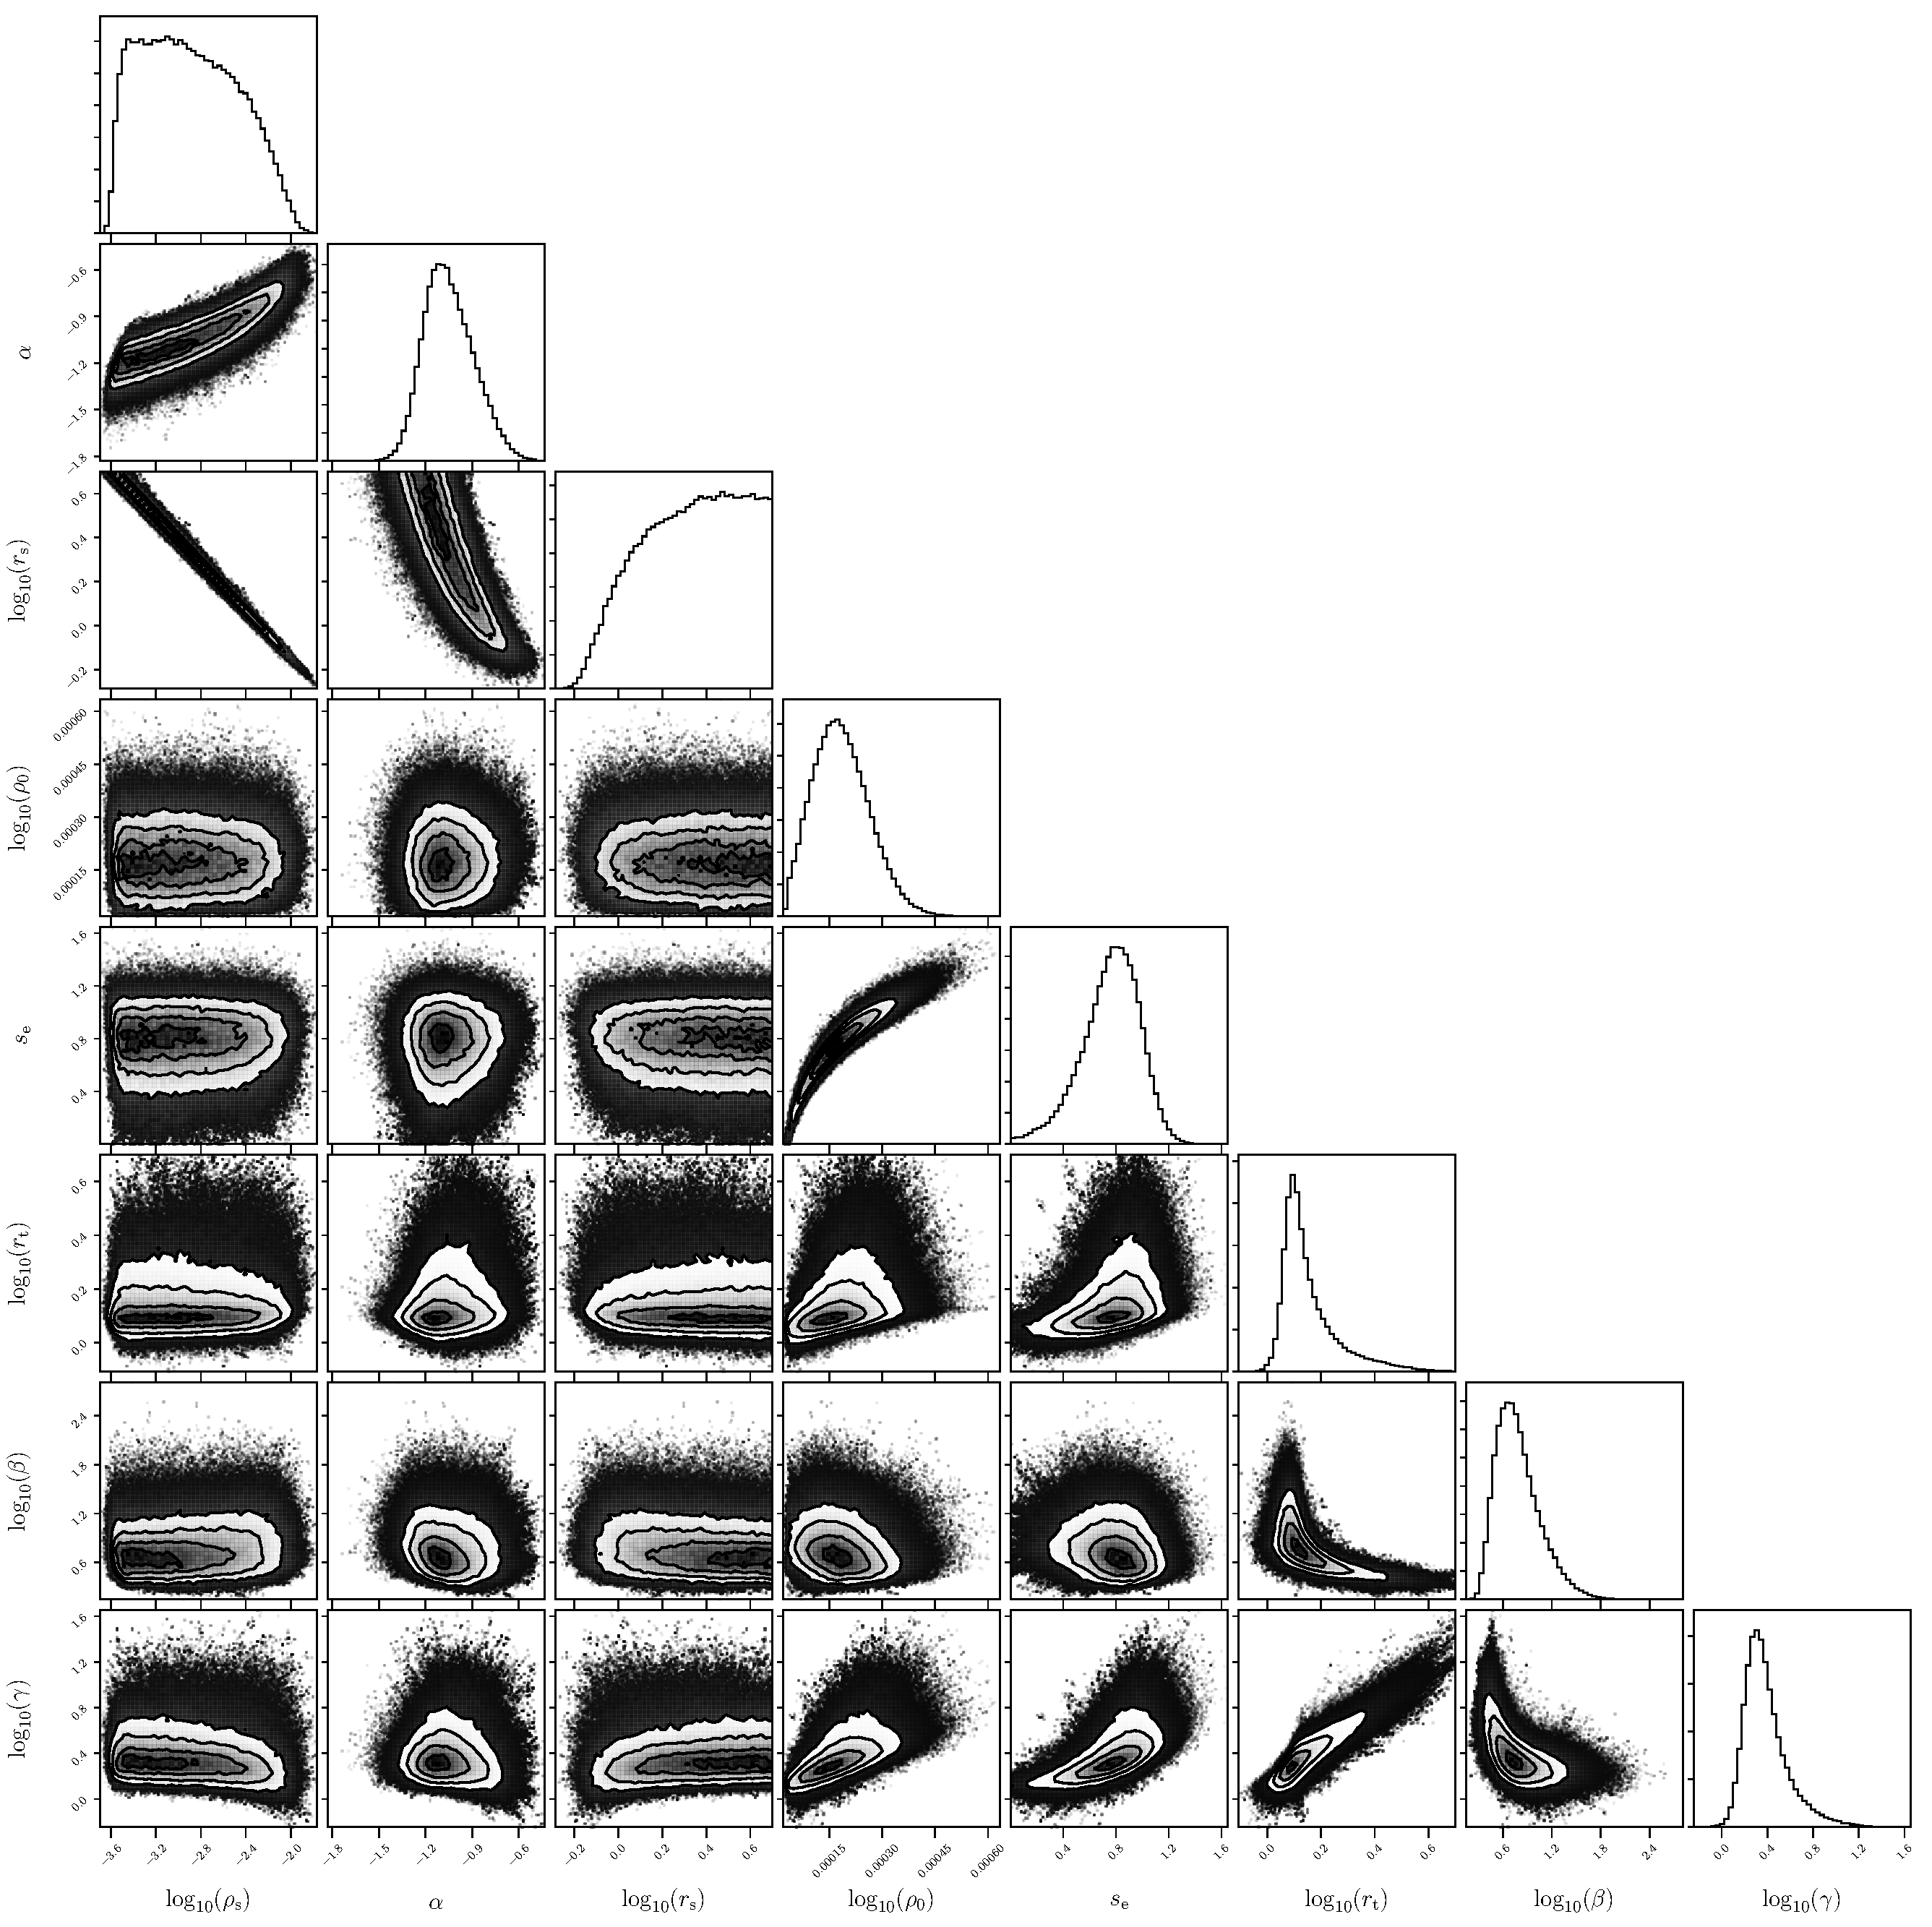
\includegraphics[width= \textwidth]{corner21.pdf}
\caption{The two-dimensional posterior distributions of each pair of
the fitting parameters corresponding to the functional
form in Equation~\ref{eq:model}. We cross-correlated PSZ2 galaxy clusters with
galaxies form the PS 21 galaxy catalog to establish this figure.}
   \label{fig:corner_21} 
\end{figure*}
\begin{figure*}
    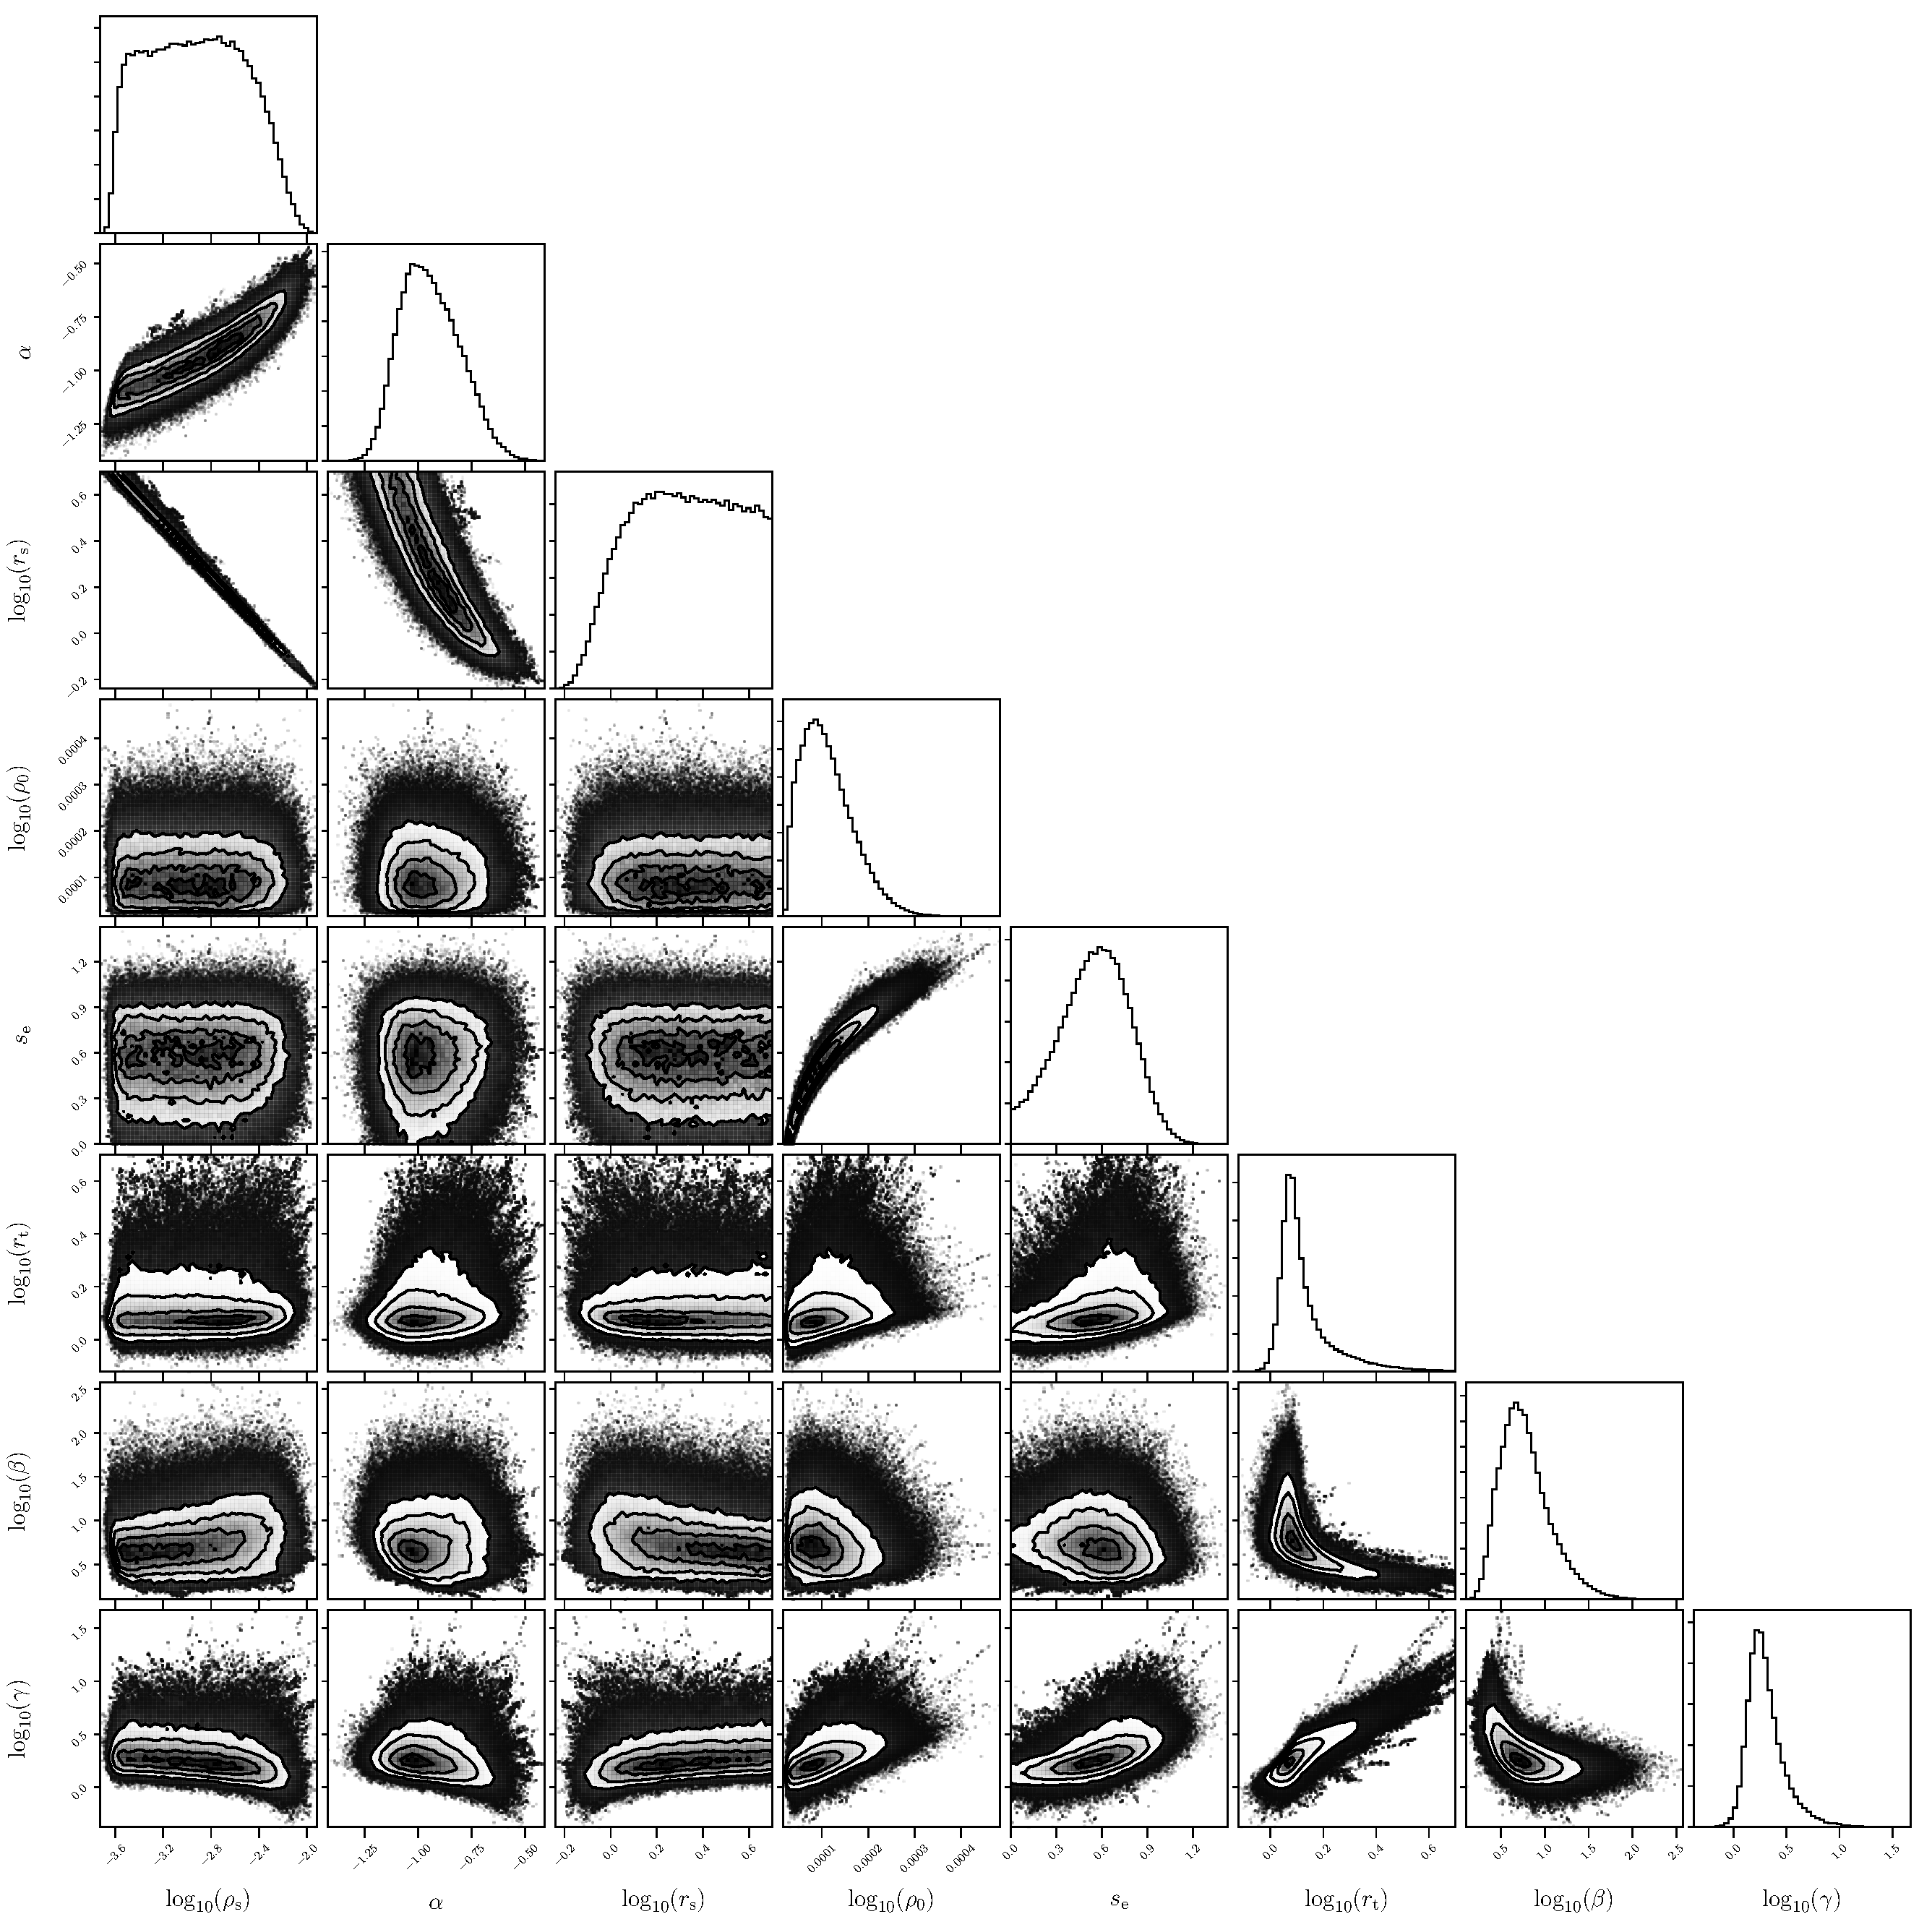
\includegraphics[width= \textwidth]{corner215.pdf}
\caption{The two-dimensional posterior distributions of each pair of
the fitting parameters corresponding to the functional
form in Equation~\ref{eq:model}. We cross-correlated PSZ2 galaxy clusters with
galaxies form the PS 21.5 galaxy catalog to establish this figure.}
   \label{fig:corner_21.5} 
\end{figure*}
\begin{figure*}
    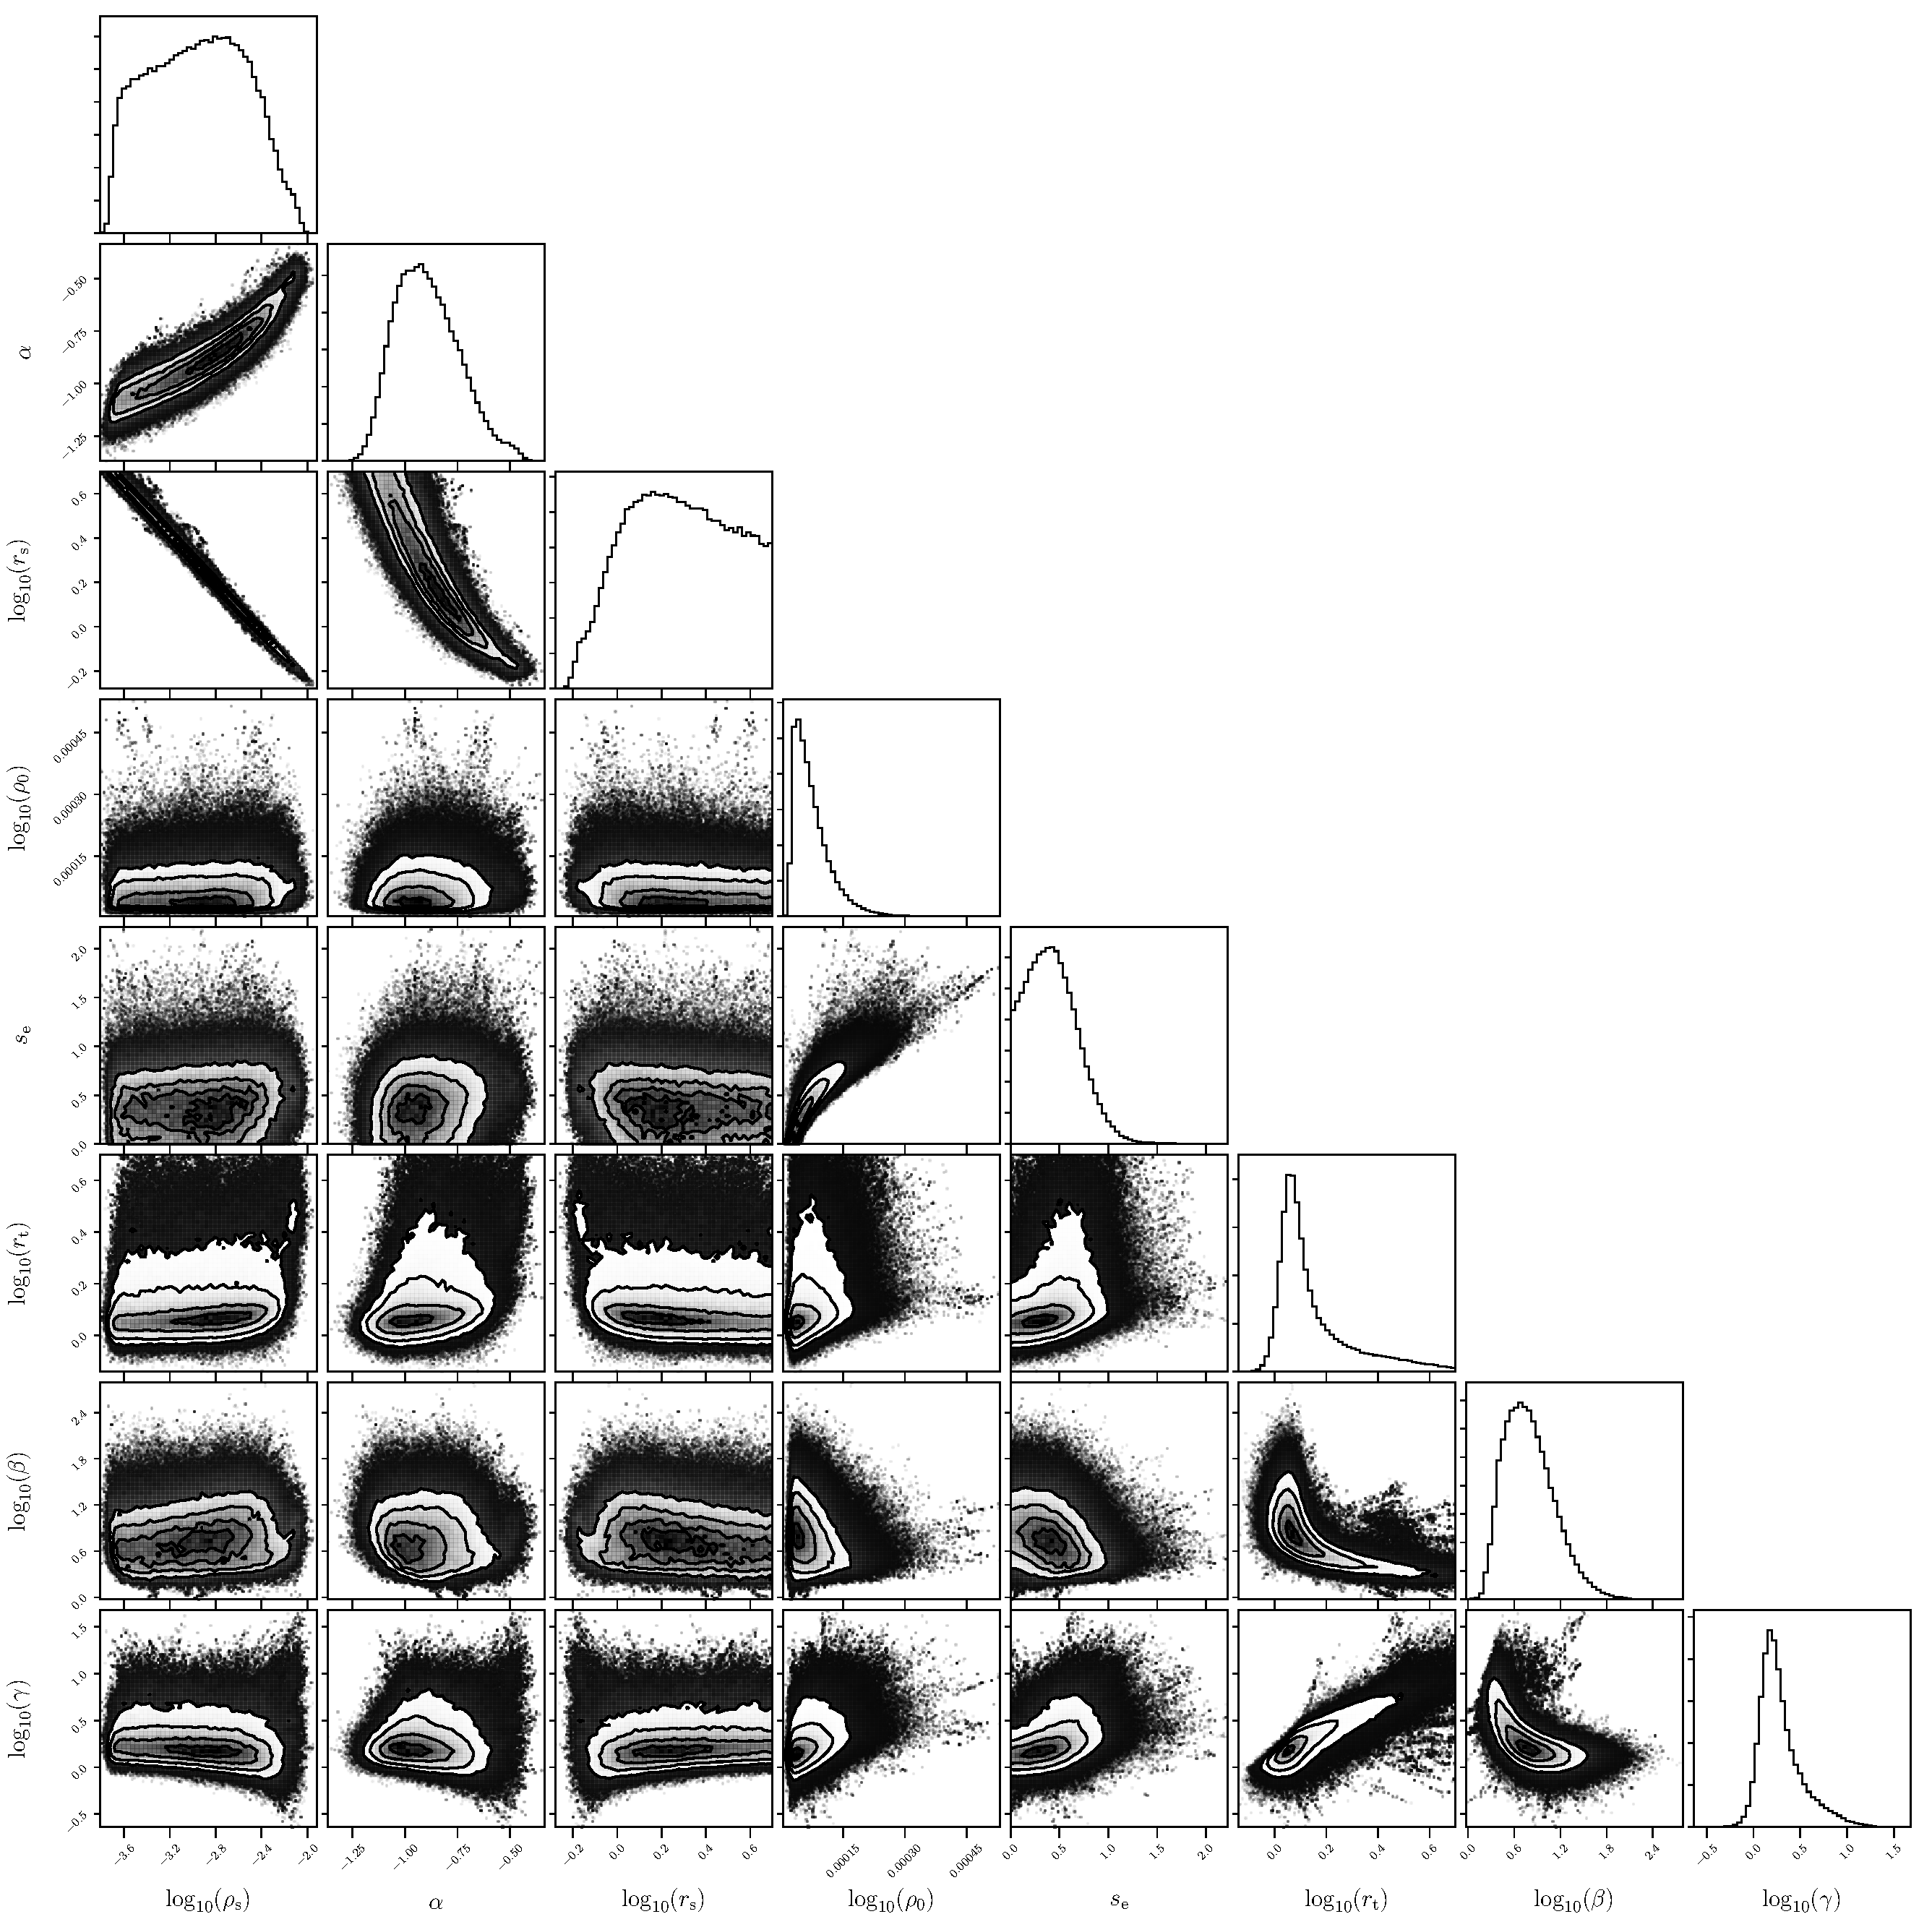
\includegraphics[width= \textwidth]{corner22.pdf}
\caption{The two-dimensional posterior distributions of each pair of
the fitting parameters corresponding to the functional
form in Equation~\ref{eq:model}. We cross-correlated PSZ2 galaxy clusters with
galaxies form the PS 22 galaxy catalog to establish this figure.}
   \label{fig:corner_22} 
\end{figure*}
\begin{figure*}
    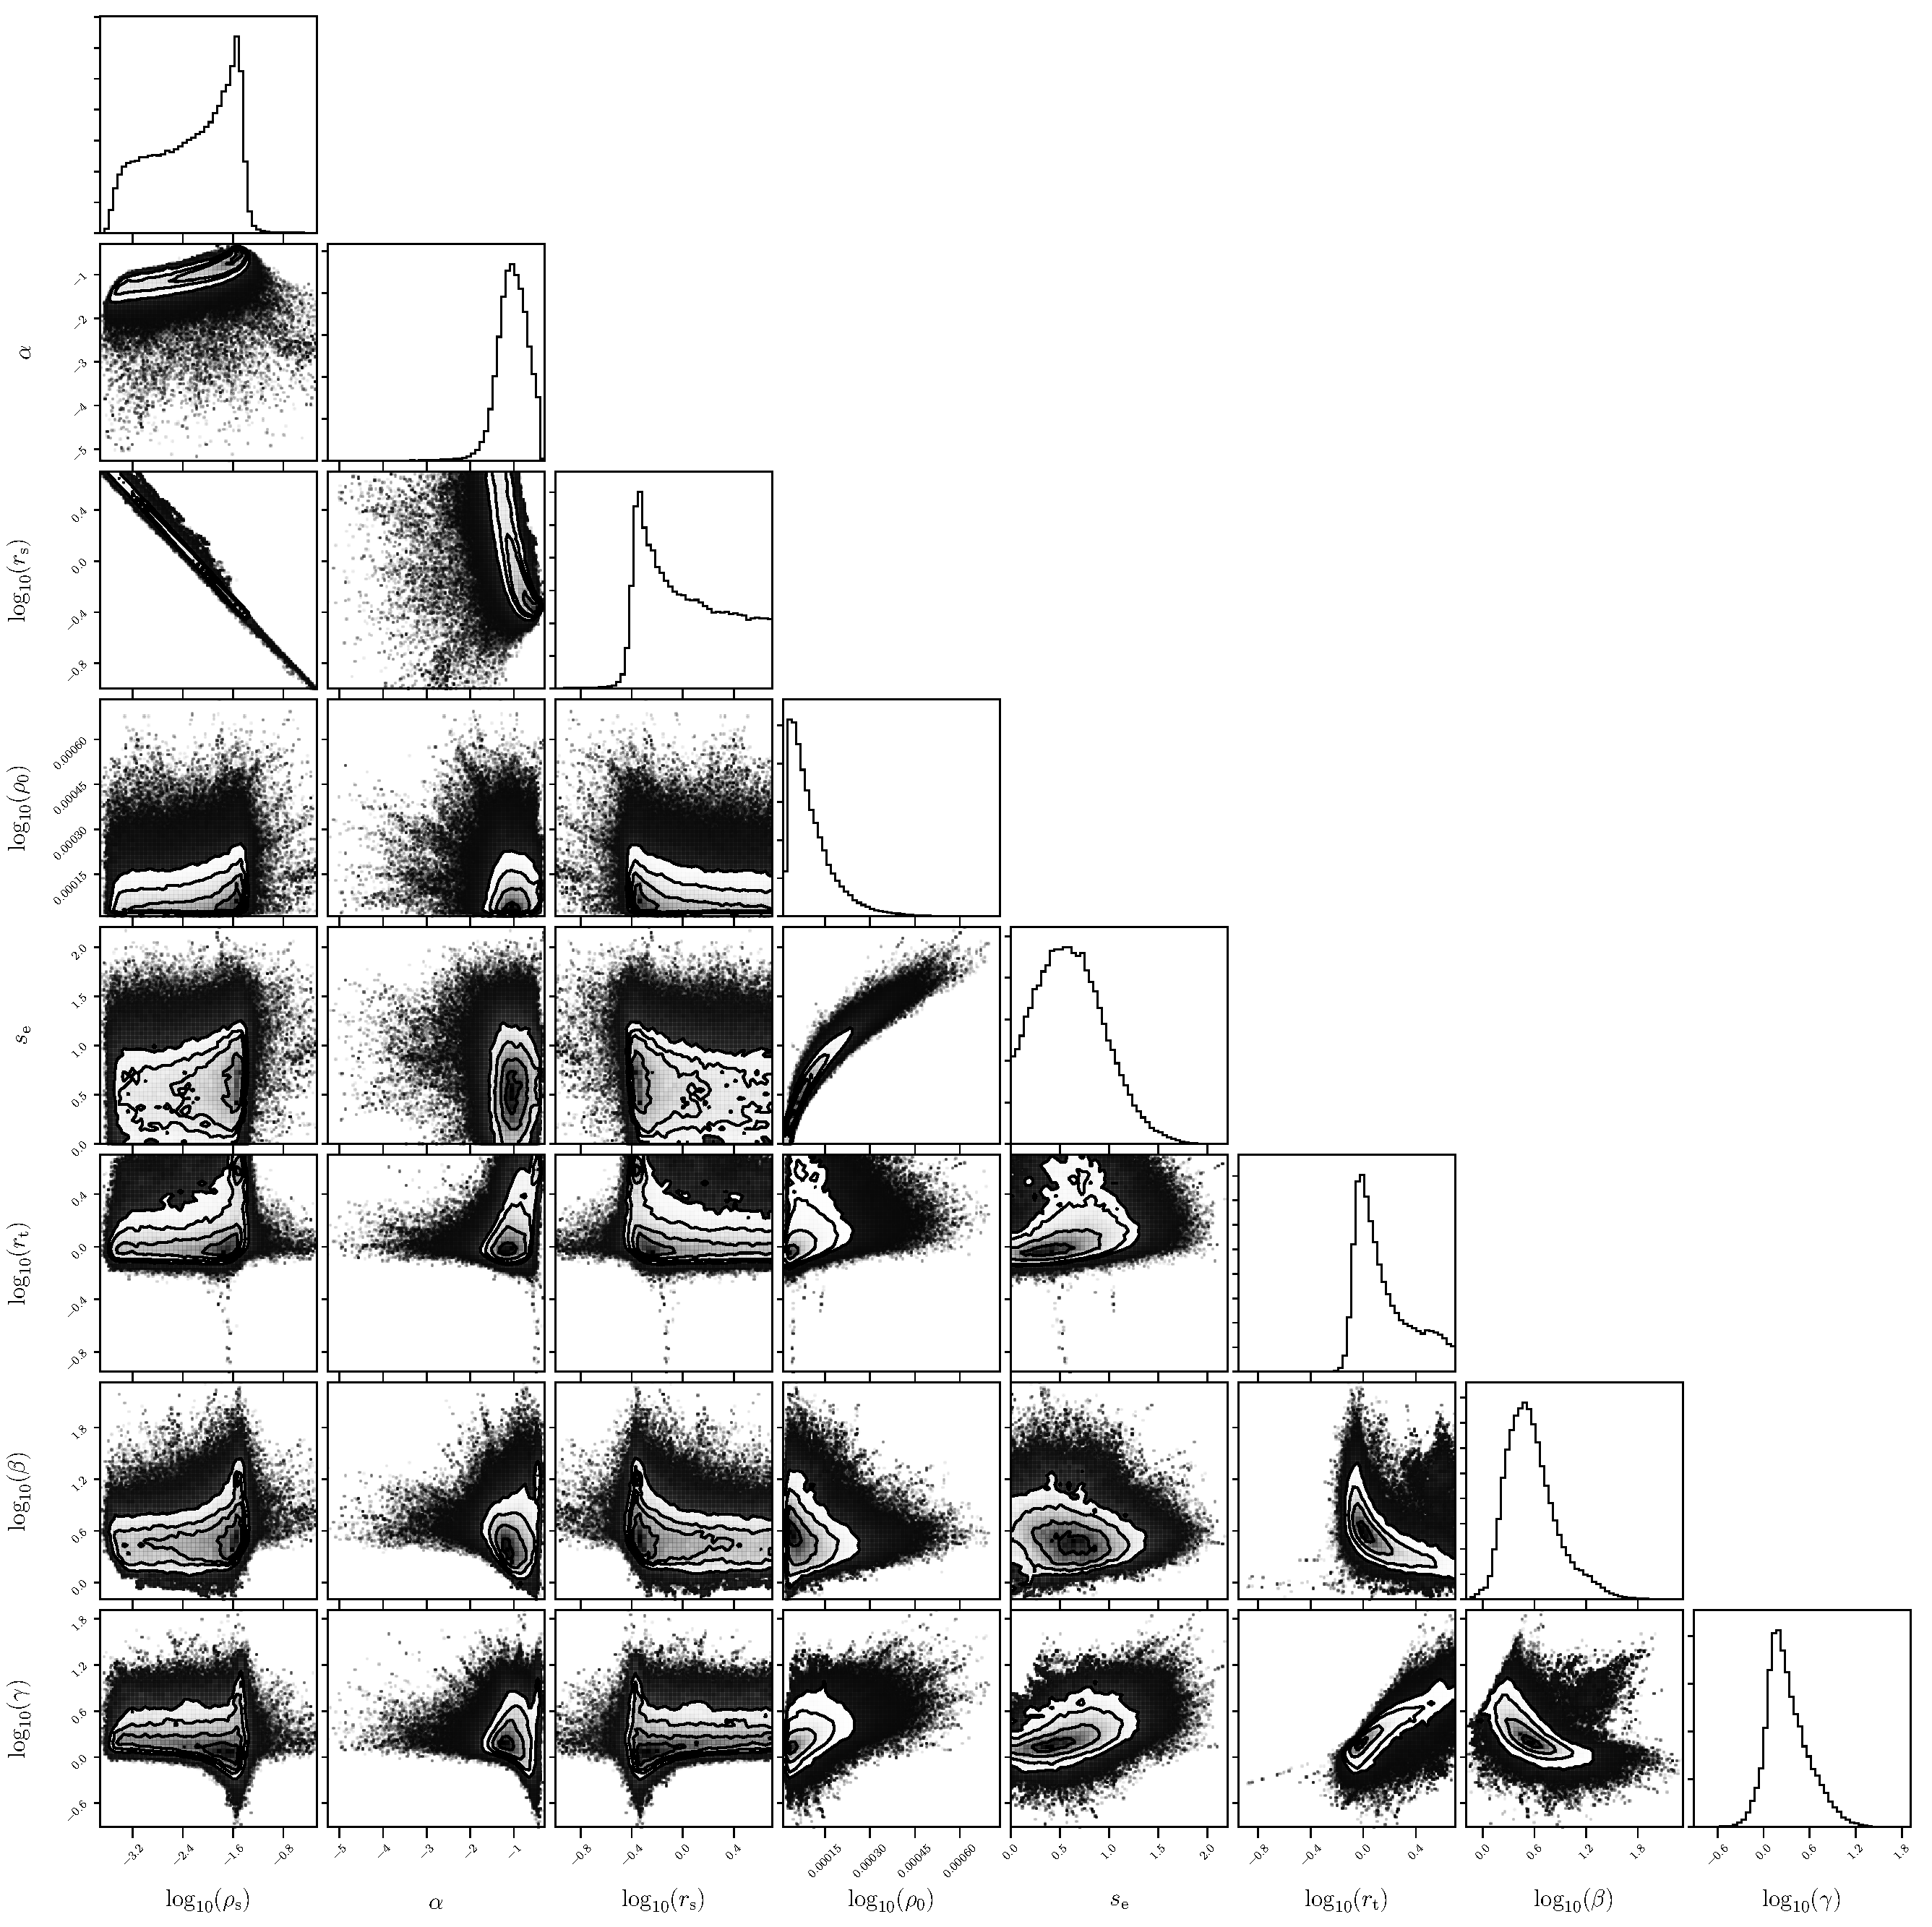
\includegraphics[width= \textwidth]{cornerred.pdf}
\caption{The two-dimensional posterior distributions of each pair of
the fitting parameters corresponding to the functional
form in Equation~\ref{eq:model}. We cross-correlated PSZ2 galaxy clusters with
galaxies form the PS 21.5 galaxy catalog. Only the galaxies labeled
as red were used.}
   \label{fig:cornerred} 
\end{figure*}
\begin{figure*}
    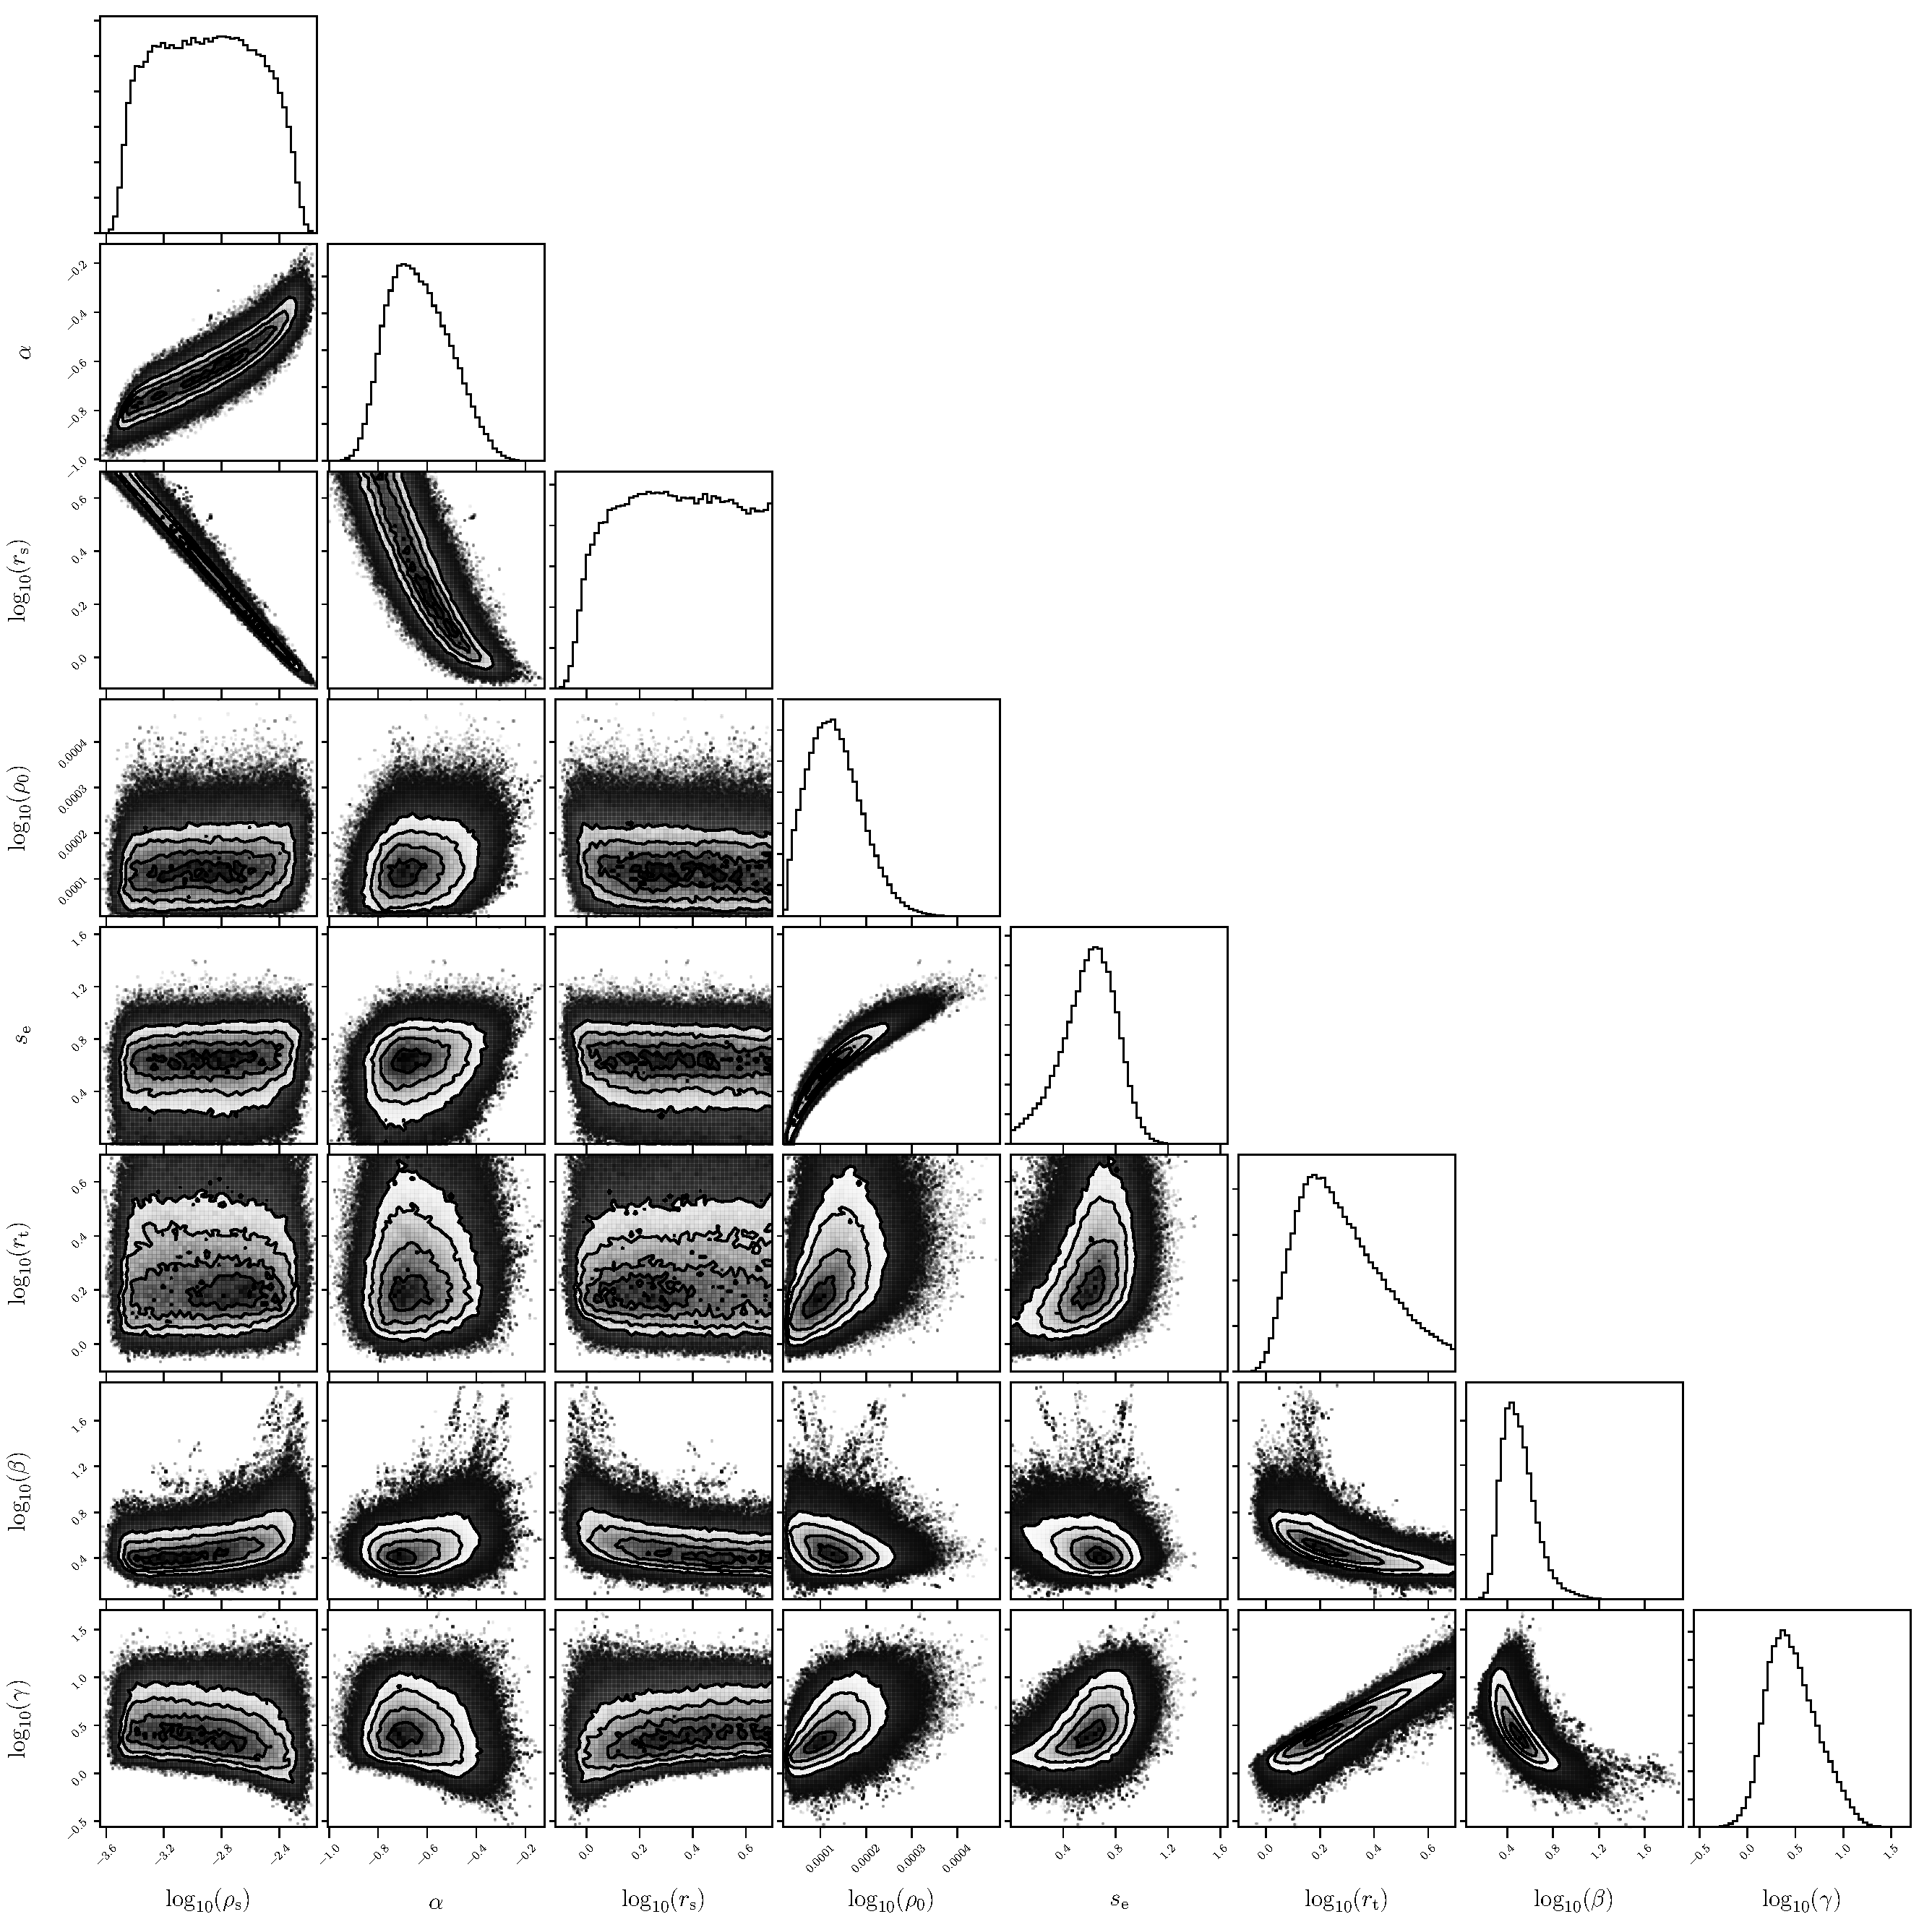
\includegraphics[width= \textwidth]{cornerblue.pdf}
\caption{The two-dimensional posterior distributions of each pair of
the fitting parameters corresponding to the functional
form in Equation~\ref{eq:model}. We cross-correlated PSZ2 galaxy clusters with
galaxies form the PS 21 galaxy catalog. Only the galaxies labeled as
blue were used.}
   \label{fig:cornerblue} 
\end{figure*}

\label{lastpage}
\end{document}
